%%Introduction

In this Section, we consider models with a photon, a W boson, a Z boson or a Higgs boson in the final state,
accompanied by Dark Matter particles that either couple directly to the boson or are mediated by
a new particle. The experimental signature is identified as \textit{V+MET}.

These models are interesting both as some are demanded by gauge coupling relations in models where the gluon provides
the experimentally detectable signature,
and also as stand-alone models with final states that cannot be generated by the models in
Section~\ref{subsec:MonojetLikeModels}.

%%%Classification of models

\begin{figure}[h!]
  \centering
  \vspace{\baselineskip}
  \unitlength=0.0045\textwidth
  \begin{feynmandiagram}[modelVisr]
    \fmfleft{i1,i2}
    \fmfright{o1,o2}
    \fmftop{isr}
    \fmfbottom{pisr}
    \fmfv{decor.shape=circle,decor.filled=shaded, decor.size=30}{v1}
    \fmf{fermion}{o2,v1,o1}
    \fmf{fermion}{i2,visr,v1}
    \fmf{plain}{v1,pvisr,i1}
    \fmf{fermion,tension=0}{v1,i1}
    \fmflabel{\Large ${\bar{q}}$}{i1}
    \fmflabel{\Large ${q}$}{i2}
    \fmflabel{\Large ${\bar{\chi}}$}{o1}
    \fmflabel{\Large ${\chi}$}{o2}
    \fmf{photon,tension=0}{visr,isr}
    \fmf{phantom,tension=0}{pvisr,pisr}
    \fmflabel{\Large ${V}$}{isr}
  \end{feynmandiagram}
  \begin{feynmandiagram}[modelVeft5pt]
    \fmfleft{i1,i2}
    \fmfright{o1,o2,o3}
    \fmf{photon,label={\Large $V$}}{v1,v2}
    \fmfv{decor.shape=circle,decor.filled=shaded, decor.size=30}{v2}
    \fmf{fermion}{i2,v1,i1}
    \fmf{fermion}{o2,v2,o1}
    \fmflabel{\Large ${\bar{q}}$}{i1}
    \fmflabel{\Large ${q}$}{i2}
    \fmflabel{\Large ${\bar{\chi}}$}{o1}
    \fmflabel{\Large ${\chi}$}{o2}
    \fmf{photon}{o3,v2}
    \fmflabel{\Large ${V}$}{o3}
  \end{feynmandiagram}
  \vspace{\baselineskip}
  \caption{Sketch of benchmark models including a contact interaction
  for V+MET searches, adapted from~\cite{Nelson:2013pqa}. \label{fig:VPlusMET_EFT}}
\end{figure}
%
The models considered can be divided in four categories:
\begin{description}
 \item[Models including a contact operator, where the boson is radiated from the initial state] As depicted in
 the top diagram of Figure~\ref{fig:VPlusMET_EFT}, these models follow the nomenclature and theory
 for the EFT benchmarks commonly used by MET+X searches~\cite{Goodman:2010ku}. These models
 have been used in past experimental searches~~\cite{Khachatryan:2014rwa, Aad:2014vka,Khachatryan:2014tva, Aad:2014vka,
 ATLAS:2014wra, Aad:2013oja}, and they will not be described here.
 \item[Models including a contact operator, where the boson is directly coupled to DM]
 Shown in the bottom of Figure~\ref{fig:VPlusMET_EFT},
 these models allow for a contact interaction vertex that directly couples the boson to Dark Matter.
 \item[Simplified models with a boson radiated either from the initial state or from the mediator] These models follow those
 already described in Section~\ref{subsec:MonojetLikeModels}, replacing the gluon with a boson.
 \item[V-specific simplified models] These models postulate direct couplings of new mediators
 to bosons, e.g. they couple the Higgs boson to a new vector or to a new scalar~\cite{Carpenter:2013xra,Berlin:2014cfa}. 
\end{description}

The following Sections describe the models within these categories,
the parameters for each of the benchmark models chosen,
the studies towards the choices of the parameters to be scanned,
and finally point to the location of their Matrix Element
implementation.

\newthought{Simplified models with ISR boson radiation}

Searches in the jet+MET final state are generally more sensitive
with respect to final states including bosons, due to the much
larger rates of signal events featuring quark or gluon radiation with
respect to radiation of bosons~\cite{Zhou:2013fla},
in combination with the low branching ratios if leptons from
boson decays are required in the final state.
The rates for the Higgs boson radiation is too low for these models
to be considered a viable benchmark~\cite{Carpenter:2013xra}.
However, the presence of photons
leptons from W and Z decays
and W or Z bosons decaying hadronically
allows to reject the background more effectively, making Z/gamma/W+MET searches
still worth comparing with searches in the jet+MET final state.

% The three commonly chosen EFT benchmarks for Dirac dark matter that are
% kinematically distinct for what concerns the observables used in
% MET+X searches~\footnote{[CD: we would need a plot here, or a reference to
% monojet section where this is shown]} and span a wide range of MET spectrum in
% the boson+MET searches are, in the notation of ~\cite{Goodman:2010ku},
% the D1 (scalar SM/WIMP interaction), D5 (vector-vector interaction) and D9
% (tensor interaction) operator.

\paragraph{Vector mediator exchanged in the s-channel}

The case for searches with W bosons in the final state has so far been strenghtened by the
presence of particular choices of couplings between the WIMP and the up and
down quarks which enhance W radiation~\cite{Bai:2012xg}, in the case of the exchange
of a vector mediator in the s-channel.
Run-1 searches have considered three sample cases for the product of
up and down quark couplings to the mediator $\xi$:
\begin{itemize}
 \item No couplings between mediator and either up or down quarks~($\xi=0$);
 \item Same coupling between mediator and each of the quark types~ ($\xi=1$);
 \item Coupling of opposite sign between mediator and each of the quark types~($\xi=-1$).
\end{itemize}
The $\xi=-1$ case leads to a large increase in the cross-section of the process,
and modifies the spectrum of missing transverse energy or
transverse mass used for the searches. The sensitivity of the W+MET search for
this benchmark in this case surpasses that of the jet+MET search.
However, as shown in Ref.~\cite{Bell:2015sza}, the cross-section increase is due
to the production of longitudinally polarized W bosons,
as a consequence of a violation of electroweak gauge symmetries. Unless further
particles are introduced (in a fashion similar
to the Higgs boson in the Standard Model), choosing a value of $\xi=-1$
for this simplified model will lead to a manifest violation of unitarity at LHC energies.
The simplified model with a vector mediator exchanged in the s-channel model
can still be considered as a benchmark for searches with a W boson if $\xi=1$.
We leave the study of further models with cross-section enhancements due
to different couplings to up and down quarks for studies beyond the early LHC searches
covered in this document.
An example of such model is the case of both DM and SM Higgs charged under a new U(1)',
with a a small mass mixing between SM Z-boson and the new Zprime. This leads
to different effective DM couplings to $u_L$ and $d_L$, proportional to
their coupling to the Z boson, detailed in Appendix~\ref{app:EWSpecificModels_Appendix}.

The scan in the parameters that characterize this simplified model for EW boson + MET
searches follow what already detailed in Section~\ref{subsec:MonojetLikeModels}.
%FIXME: refer to appropriate subsection

% CD: I tend to like this list so I'll leave it here in hope of recycling it
% \begin{itemize}
%  \item the mass of the DM particle ($m_{DM}$);
%  \item the mediator mass ($m_{Med}$);
%  \item the mediator width ($\Gamma_{Med}$);
%  \item the couplings between the DM and the mediator (\gdm),
%  and between the mediator and the initial state quarks ($g_{SM}$);
%  \item the chirality of the couplings between DM and mediator,
%  and between mediator and initial state quarks (vector-vector, axial-vector, axial-axial, vector-axial).
% \end{itemize}

As in the case of the jet+MET models, the width does not have a significant
impact on the kinematic distributions relevant for those searches. An example
of the particle-level analysis acceptance using the
generator-level cuts from Ref.~\cite{Aad:2014tda}
for the photon+MET analysis, but raising the photon $p_T$ cut
to 150 GeV is shown in Figure~\ref{fig:DMV_EW_gamma_acceptance},
comparing a width that is set to $\Gamma=M_{med}/3$ to the
minimal width (the ratio between the two widths
ranges from 1.05 to 1.5 with increasing mediator masses).

% mmed : minW
% 10  : 3.5
% 50 : 21.3
% 100 : 42.4
% 300 : 127.3
% 600 : 300.1
% 1000 : 503
% 3000 : 1512
% 6000 : 3024

\begin{figure}
    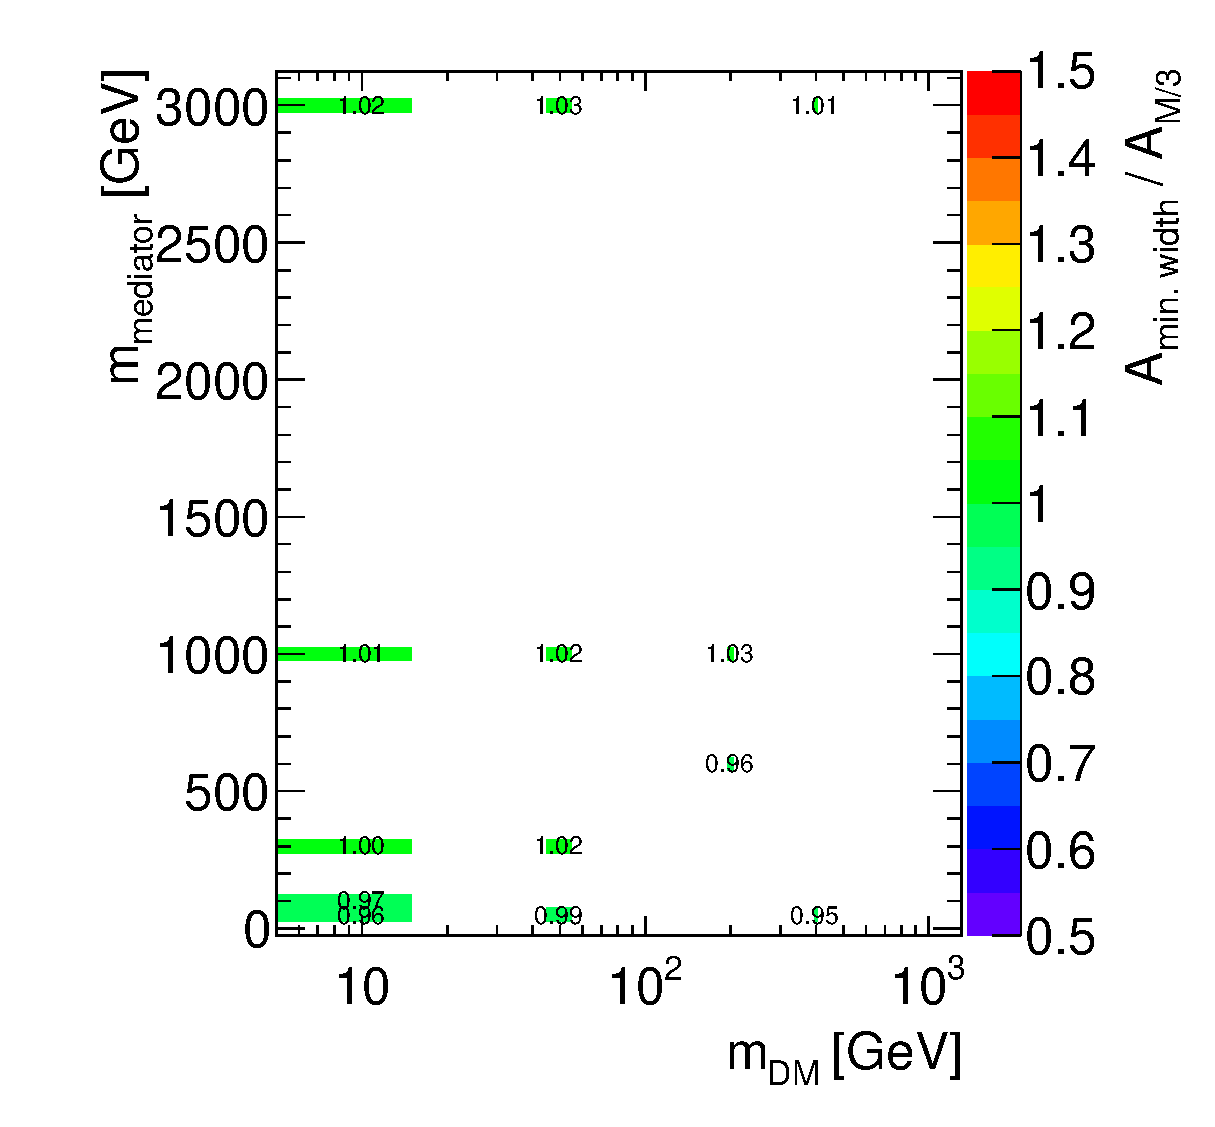
\includegraphics[width=0.7\textwidth]{figures/EW/acceptance_minwidth_vs_mo3_gamma}
    \caption{Analysis acceptance for the photon+MET analysis when varying the mediator width, in the
    case of a vector mediator exchanged in the $s-$channel}%This plot will come from Marie-Helene
    \label{fig:DMV_EW_gamma_acceptance}
\end{figure}

Examples of relevant kinematic distributions for selected benchmark points are
shown in Fig.~\ref{fig:DMV_EW_kinematics};
leading-order cross-sections for the chosen
benchmark points are shown in Table~\ref{table:x-sec}
\textbf{[TODO: Insert table of cross-sections]}.

\begin{figure}[h!]
  \centering
  \subfloat[Missing transverse momentum distribution for the photon+MET final state, for
  different mediator mass choices, for a DM mass of 10 GeV.\label{fig:DMV_EW_gamma_MET}]{%
      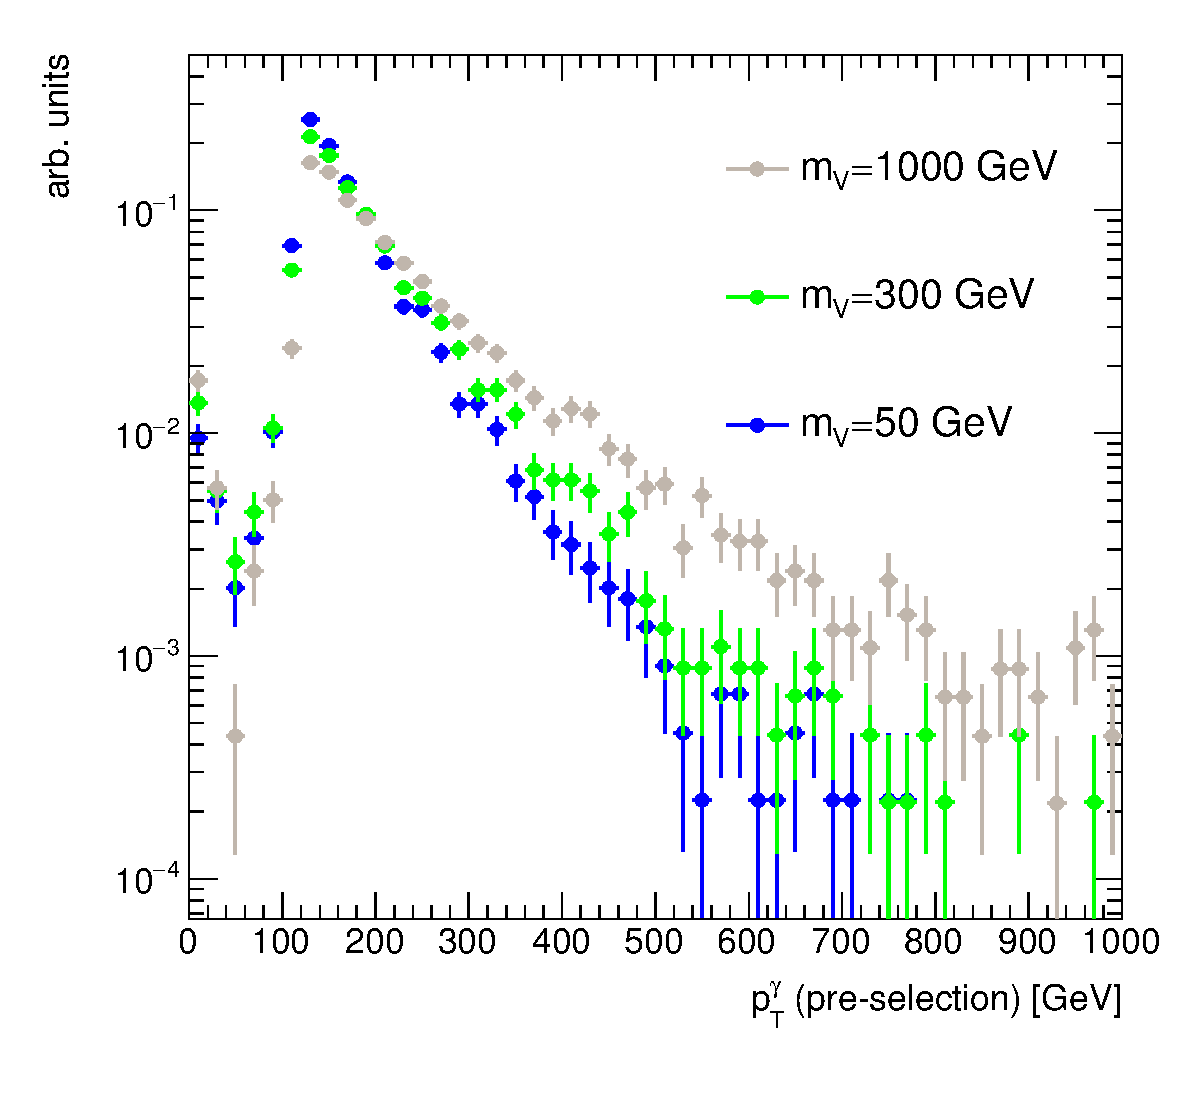
\includegraphics[width=0.45\textwidth]{figures/EW/ptGamma_filter120GeV_dmV_dm10GeV}
    }%TODO: add equivalent plot of MET to appendix
    \hfill
  \subfloat[Leading photon transverse momentum distribution for the photon+MET final state,
  for different DM mass choices, with a mediator mass of 1 TeV.\label{fig:DMV_EW_gamma_pT}]{%
      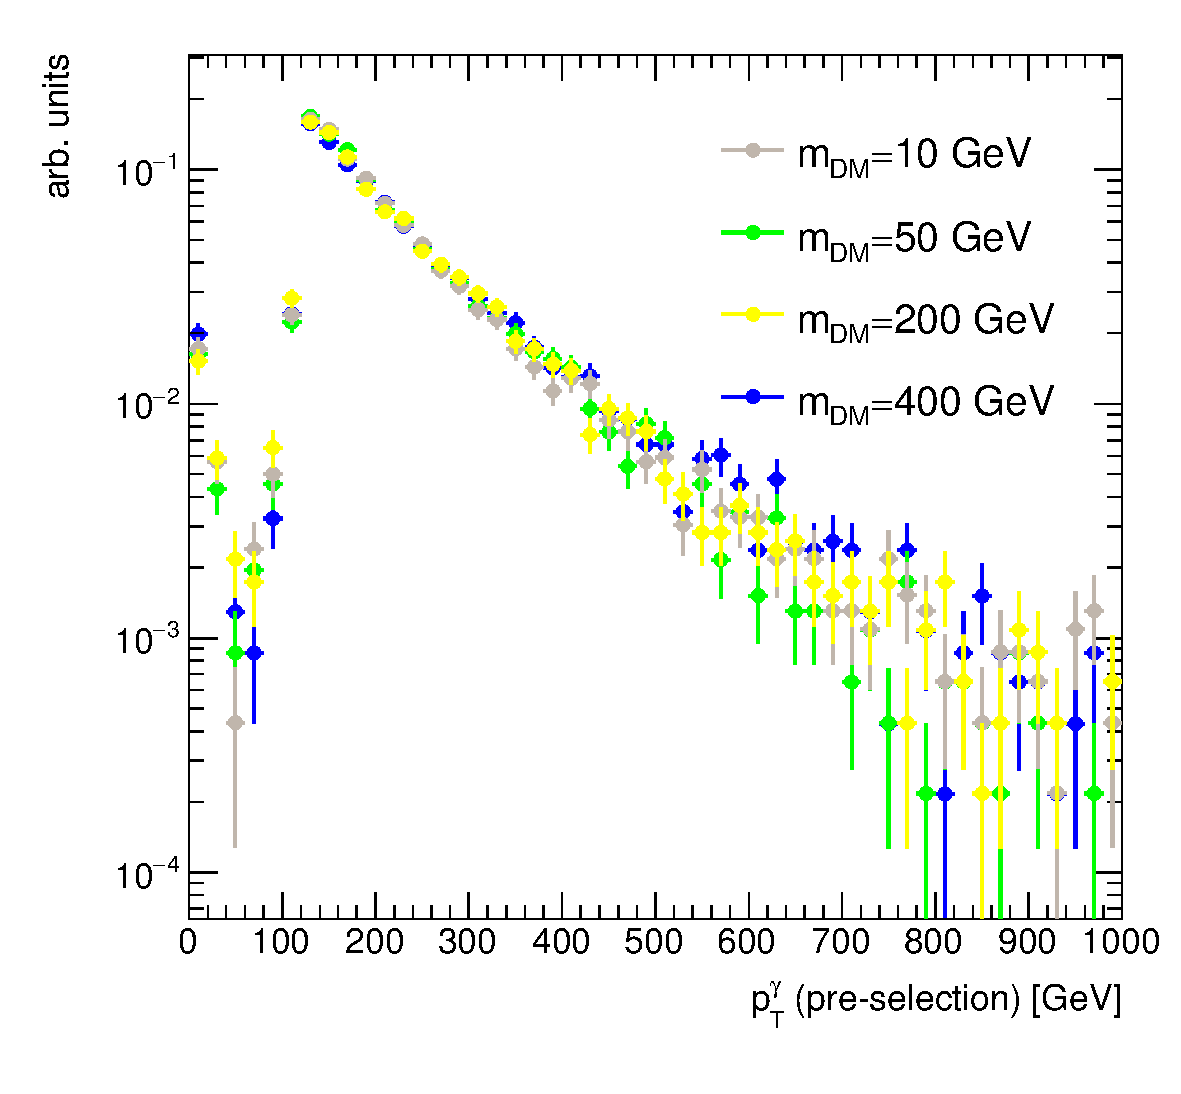
\includegraphics[width=0.45\textwidth]{figures/EW/ptGamma_filter120GeV_dmV_mV1000GeV}
    }%TODO: add equivalent plot of MET to appendix
    \hfill
  \subfloat[Missing transverse momentum distribution for the leptonic Z+MET final state.\label{fig:DMV_EW_Z_MET}]{%
      
\includegraphics[width=0.45\textwidth]{figures/llug}
    }
  \subfloat[Transverse mass ($m_T$) for the leptonic W+MET final state.\label{fig:DMV_EW_Wlep_mT}]{%
      
\includegraphics[width=0.45\textwidth]{figures/gull}
    }
    \hfill
  \subfloat[Missing transverse momentum distribution for the hadronic W+MET final state.\label{fig:DMV_EW_Whad_MET}]{%
      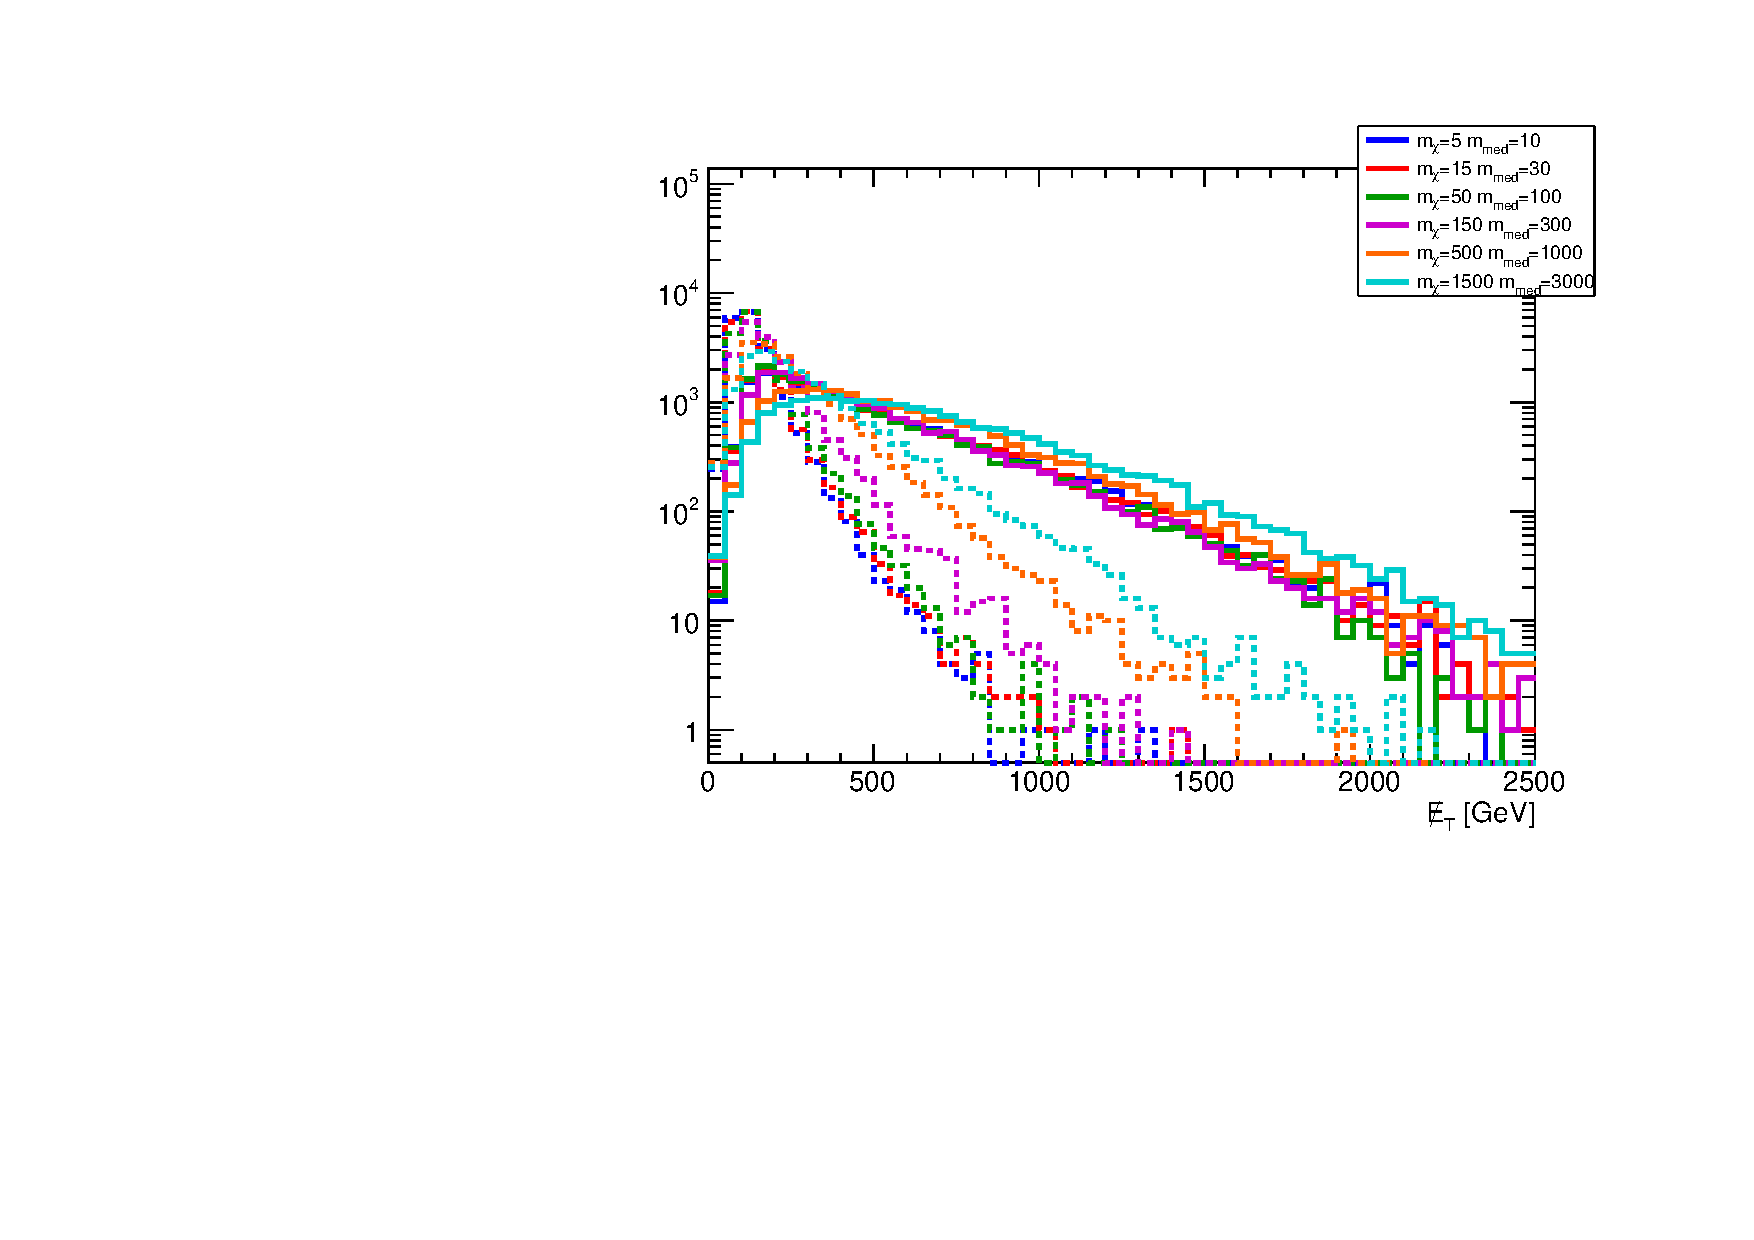
\includegraphics[width=0.45\textwidth]{figures/EW/monoWhad_Destructive/metPt}
    }
    \caption{Kinematic distributions relevant for searches with W, Z and photons in the final state,
    for the simplified model with a vector mediator exchanged in the $s-$channel.}
    \label{fig:DMV_EW_kinematics}
\end{figure}

\paragraph{Colored scalar mediator exchanged in the s-channel}

t-channel colored scalar, to be completed...

\paragraph{Model implementation}

These models are generated at leading order with MadGraph 2.2.2, and parameter
cards can be found on SVN \textbf{[TODO: Add SVN location]}.
The parton shower is done using Pythia 8, with a matching scale of...
\textbf{[TODO: To be completed.]}

% +++++++++++++++++++++++++++++++++++++++++++++++++++++++++++++++++++++++++++++++++++++
% Linda 11/5/2015
% +++++++++++++++++++++++++++++++++++++++++++++++++++++++++++++++++++++++++++++++++++++

\newthought{EFT models with direct DM-boson couplings}

A complete list of effective operators with direct DM/boson couplings for
Dirac DM, up to dimension 7, can be found in~\cite{Cotta:2012nj}.

The lowest dimension benchmark operators we may consider are effective dimension 5.  Following the notation of~\cite{Carpenter:2012rg},  models
from this category have a Lagrangian that includes terms such as:

\begin{eqnarray}
\frac{m_W^2}{\Lambda_5^3} ~\bar{\chi} \chi ~W^{+ \mu} W^{-}_\mu
+ \frac{m_Z^2}{2 \Lambda_5^3} ~ \bar{\chi} \chi ~ Z^\mu Z_\mu ~.
\end{eqnarray}

where $m_Z$ and $m_W$ are the masses of the $Z$ and $W$ boson, $W^{\mu}$ and $Z^{\mu}$
are the fields of the gauge bosons, $\chi$ denote the Dark Matter fields
and $\Lambda_5$ is the effective field theory scale.  Note that these operators are of true dimension 7, 
but reduce to effective dimension 5 once Higgs vevs, contained in the W and Z mass terms, are inserted.  
As such , one expects  these that operators would naturally  arise in UV complete models where Dark Matter 
interacts via a Higgs portal where heavy mediators would couple to the Higgs or other fields in an extended Higgs sector. 
In such models the full theory may be expected to contain additional operators with Higgs-Dark Matter couplings. 
Concentrating  for the moment on mono-gauge boson signals, the above operator induces signatures with 
MET in conjunction with Z and W bosons at tree level,
while at loop level it induces couplings to photon pairs and $Z \gamma$ through W loops.
In these models, a clear relation exists between final states with photons, EW bosons
and Higgs boson. \textbf{[TODO: see if mono-Higgs studies exist for these operators, include them here]}.

% +++++++++++++++++++++++++++++++++++++++++++++++++++++++++++++++++++++++++++++++++++++
% Uli 3/5/2015
% +++++++++++++++++++++++++++++++++++++++++++++++++++++++++++++++++++++++++++++++++++++

The dimension-7 benchmark models  contain the $SU(2)_L \times U(1)_Y$ gauge-invariant couplings between DM fields and the kinetic terms of the EW bosons. The CP-conserving scalar couplings of this type can be written as
\begin{equation} \label{eq:Lc1c2}
\frac{c_1}{\Lambda_S^3} \, \bar \chi \chi \, B_{\mu \nu} B^{\mu \nu }  + \frac{c_2}{\Lambda_S^3} \, \bar \chi \chi \, W_{\mu \nu}^i W^{i, \mu \nu }  \,.
\end{equation}
Here $B_{\mu \nu} = \partial_\mu B_\nu - \partial_\nu B_\mu$ and $W_{\mu \nu}^i =  \partial_\mu W_\nu^i - \partial_\nu W_\mu^i + g_2 \hspace{0.25mm} \epsilon^{ijk}  \hspace{0.25mm}  W_\mu^j \hspace{0.25mm} W_\mu^k$ are the $U(1)_Y$ and $SU(2)_L$ field strength tensor, respectively, and  $g_2$ denotes the weak coupling constant. In the case of the pseudoscalar couplings, one has instead
\begin{equation} \label{eq:Lc3c4}
\frac{c_1}{\Lambda_P^3} \, \bar \chi \gamma_5 \chi \, B_{\mu \nu} \tilde B^{\mu \nu }  + \frac{c_2}{\Lambda_P^3} \, \bar \chi \gamma_5 \chi \, W_{\mu \nu}^i \tilde W^{i, \mu \nu }  \,,
\end{equation}
where $\tilde B_{\mu \nu} = 1/2 \hspace{0.5mm} \epsilon_{\mu \nu  \lambda \rho}  \hspace{0.25mm}  B^{\lambda \rho}$ and $\tilde W_{\mu \nu}^i = 1/2 \hspace{0.5mm} \epsilon_{\mu \nu  \lambda \rho}  \hspace{0.25mm}  W^{i, \lambda \rho}$ are the dual  field strength tensors. In addition to the CP-conserving interactions (\ref{eq:Lc1c2}) and (\ref{eq:Lc3c4}), there are also four CP-violating couplings that are obtained from the above operators by the replacement $\bar \chi \chi \leftrightarrow \bar \chi \gamma_5 \chi$.

The effective interactions introduced in (\ref{eq:Lc1c2}) and  (\ref{eq:Lc3c4}) appear  in models of Rayleigh DM~\cite{Weiner:2012cb}. Ultraviolet completions where the operators are generated through loops of states charged under $U(1)_Y$ and/or $SU(2)_L$  have been proposed in \cite{Weiner:2012gm} and their LHC signatures have been studied in \cite{Liu:2013gba}. If these new charged particles  are  light, the high-$p_T$ gauge bosons that participate in  the MET processes considered here are able to resolve the substructure of the loops. This generically suppresses the cross sections compared to the EFT predictions~\cite{Haisch:2012kf}, and thus will weaken the bounds on the interaction strengths of  DM and the EW gauge bosons  to some extent.  Furthermore, the light charged mediators may be produced  on-shell in $pp$ collisions, rendering direct LHC searches potentially more restrictive than MET searches. Making the above statements precise would require further studies beyond the timescale of this forum.

Since for $\Lambda_S = \Lambda_P$ the effective interactions (\ref{eq:Lc1c2}) and (\ref{eq:Lc3c4}) predict essentially the same value of the mono-photon, mono-$Z$ and mono-$W$ cross section \cite{Carpenter:2012rg,Crivellin:2015wva}, we consider below only the former couplings. We emphasise however that measurements of the jet-jet azimuthal angle difference in  MET$+ 2 j$ events may be used to disentangle whether DM couples more strongly to the combination $B_{\mu \nu} B^{\mu \nu}$ ($W_{\mu \nu}^i W^{i, \mu \nu }$) or the product $B_{\mu \nu} \tilde B^{\mu \nu}$ ($W_{\mu \nu}^i \tilde W^{i, \mu \nu }$) of field strength tensors \cite{Cotta:2012nj,Crivellin:2015wva}.


After EW symmetry breaking the interactions (\ref{eq:Lc1c2}) induce direct couplings between pairs of DM particles and  gauge bosons.  The corresponding Feynman rule reads
\begin{equation}  \label{eq:feynman}
\frac{4 \hspace{0.25mm} i}{\Lambda_S^3} \; g_{V_1 V_2} \, \big (  p_1^{\mu_2} \hspace{0.25mm} p_2^{\mu_1} - g^{\mu_1 \mu_2}  \, p_1 \cdot p_2 \big ) \,,
\end{equation}
where $p_i$ ($\mu_i$) denotes the momentum (Lorentz index) of the vector field $V_i$ and for simplicity the spinors associated with the DM fields have been dropped. The couplings $g_{V_i V_j}$ take the form
\begin{equation} \label{eq:gViVj}
\begin{split}
g_{\gamma \gamma} & = c_w^2 \hspace{0.25mm} c_1+ s_w^2  \hspace{0.25mm} c_2 \,, \\[1mm]
g_{\gamma Z}   & = - s_w c_w \, \big (  c_1  - c_2  \big ) \,, \\[1mm]
g_{ZZ}  & = s_w^2 \hspace{0.25mm} c_1 + c_w^2  \hspace{0.25mm} c_2  \,, \\[1mm]
g_{WW} & = c_2 \,,
\end{split}
\end{equation}
with $s_w$ ($c_w$) the sine (cosine) of the weak mixing angle. Note that our coefficients $c_1$ and $c_2$ are identical to the coefficients $C_B$ and $C_W$ used in \cite{Crivellin:2015wva}, while they are related via $k_1 = \frac{1}{{c_w}^2} c_1$ and $k_2 = \frac{1}{{s_w}^2} c_2$ to the coefficients $k_1$ and $k_2$ introduced in \cite{Carpenter:2012rg}.

The coefficients $c_1$ and $c_2$ appearing in (\ref{eq:gViVj}) determine the relative importance of each of the MET channels and their correlations. For example, one observes that:
\begin{itemize}
 \item Only $c_2$ enters the coupling between DM and $W$ bosons, meaning that only models with $c_2 \neq 0$ predict a mono-$W$ signal;
 \item If $c_1 = c_2$ the mono-photon (mono-$Z$) signal does not receive contributions from diagrams involving $Z$ (photon) exchange;
  \item Since numerically $c_w^2/s_w^2 \simeq 3.3$ the mono-photon channel is particularly sensitive to $c_1$.
\end{itemize}




% +++++++++++++++++++++++++++++++++++++++++++++++++++++++++++++++++++++++++++++++++++++
% +++++++++++++++++++++++++++++++++++++++++++++++++++++++++++++++++++++++++++++++++++++

As shown in Fig.~\ref{fig:EW_EFT5_Zlep_MET}
kinematics of this model can be approximated by that of a simplified model including
a high-mass scalar mediator exchanged in the s-channel. For this reason,
the list of benchmark models with direct boson-DM couplings only includes dimension 7 operators.
\textbf{[TODO: then we need to recommend the scalar mediator,
but then the sensitivity is very poor wrt monojets - however, I still prefer
to generate a few (high-mass) simplified model points wrt an EFT if given the choice.]}

\begin{figure}
    
\includegraphics[width=0.6\textwidth]{figures/gull}
    \caption{Comparison of the missing transverse momentum for the simplified model
    where a scalar mediator is exchanged in the s-channel and the model including
    a dimension-5 scalar contact operator, in the leptonic Z+MET final state}
    \label{fig:EW_EFT5_Zlep_MET}
\end{figure}

The kinematic distributions for dimension-7 scalar and pseudoscalar operators
only shows small differences, as shown in Fig.~\ref{fig:EW_EFT5_gamma_MET}.

\begin{figure}
    
\includegraphics[width=0.6\textwidth]{figures/llug}
    \caption{Comparison of the missing transverse momentum for the scalar and pseudoscalar
    operators with direct interaction between DM and photon, in the photon+MET final state}
    \label{fig:EW_EFT5_gamma_MET}
\end{figure}

Similarly, the differences in kinematics for the various signatures
are negligible when changing the coefficients $k_1$ and $k_2$, as shown
in Figure~\ref{EFTD7_EW_kinematics}. Only the case $k_1=k_2=1$ is generated as benchmark;
other cases are left for reinterpretation as they will only need a rescaling of the cross-sections
shown in Table~\ref{} \textbf{[TODO: add tables with cross sections]} for the various Dark Matter
mass points considered.

\begin{figure}[h!]
  \centering
  \subfloat[Missing transverse momentum distribution for the photon+MET final state.\label{fig:EFTD7_EW_gamma_MET}]{%
      
\includegraphics[width=0.45\textwidth]{figures/gull}
    }
    \hfill
  \subfloat[Missing transverse momentum distribution for the leptonic Z+MET final state.\label{fig:EFTD7_EW_Z_MET}]{%
      
\includegraphics[width=0.45\textwidth]{figures/llug}
    }
  \subfloat[Transverse mass ($m_T$) for the leptonic W+MET final state.\label{fig:EFTD7_EW_Wlep_mT}]{%
      
\includegraphics[width=0.45\textwidth]{figures/gull}
    }
    \caption{Kinematic distributions relevant for searches with W, Z and photons in the final state,
    for for the scalar and pseudoscalar operators representing direct interactions between DM and bosons.}
    \label{fig:EFTD7_EW_kinematics}

\end{figure}

Examples of relevant kinematic distributions for selected benchmark points are
shown in Fig.~\ref{fig:DMV_EW_kinematics}.

\begin{figure}[h!]
  \centering
  \subfloat[Missing transverse momentum distribution for the photon+MET final state.\label{fig:DMV_EW_gamma_MET}]{%
      
\includegraphics[width=0.45\textwidth]{figures/gull}
    }
    \hfill
  \subfloat[Missing transverse momentum distribution for the leptonic Z+MET final state.\label{fig:DMV_EW_Z_MET}]{%
      
\includegraphics[width=0.45\textwidth]{figures/llug}
    }
  \subfloat[Transverse mass ($m_T$) for the leptonic W+MET final state.\label{fig:DMV_EW_Wlep_mT}]{%
      
\includegraphics[width=0.45\textwidth]{figures/gull}
    }
    \hfill
  \subfloat[Fat \textbf{[Insert algorithm]} jet mass ($m_T$) for the the hadronic W+MET final state.\label{fig:DMV_EW_Whad_jetMass}]{%
      
\includegraphics[width=0.45\textwidth]{figures/llug}
    }
    \caption{Kinematic distributions relevant for searches with W, Z and photons in the final state,
    for the simplified model with a vector mediator exchanged in the $s-$channel.}
    \label{fig:DMV_EW_kinematics}
\end{figure}

\paragraph{Completion and validity of EW contact operators}

\textbf{[TODO: mention here discussion with Liantao yesterday]}

% +++++++++++++++++++++++++++++++++++++++++++++++++++++++++++++++++++++++++++++++++++++
%   Linda 11/5/15
% +++++++++++++++++++++++++++++++++++++++++++++++++++++++++++++++++++++++++++++++++++++

As an example of a simplified model corresponding to the dimension-5 EFT operator 
described above, we consider a Higgs portal with a scalar mediator. Models of this kind
are among the most concise versions of simplified models that produce 
couplings of Dark Matter to pairs of gauge-bosons.  Scalar fields may couple directly to pairs of electroweak gauge bosons, 
but must carry part of the electroweak vev.  One may thus consider a simple model where Dark Matter couples to a a scalar 
singlet mediator, which mixes with the fields in the Higgs sector.
\begin{equation}
L\subset m_s S^2 + \lambda S^2H^2 +\lambda^{'} S H^2 + y S \chi \overline{\chi}
\end{equation}
Where H is a field in the Higgs sector that contains part of the electroweak vev, 
S is a heavy scalar singlet and $\chi$ is a Dark Matter field. 
There is then an S channel diagram where DM pairs couple to the singlet field S, 
which then mixes with a Higgs-sector field, and couples to W and Z bosons. 
This diagram contains 2 insertions of EW symmetry breaking fields, 
corresponding in form to the effective dimension-5 operator in the previous section.   

\paragraph{Model implementation}

The model can be found on the Forum SVN repository~\cite{ForumSVN_monoHEFTD5}.

\newthought{Specific simplified models including EW bosons}

Three benchmark simplified models \cite{Carpenter:2013xra,Berlin:2014cfa} 
are recommended for MET+Higgs searches:
\begin{itemize}
	\item A model where a vector mediator ($Z_B'$) is exchanged in the $s-$channel, 
	radiates a Higgs or a $Z$ boson and decays into two DM particles;
	\item A model where a scalar mediator $S$ couples to the SM only 
	through the SM Higgs and decays to two DM particles;
	\item A model where a vector $Z'$ is produced resonantly and decays into a Higgs boson
	plus an intermediate heavy pseudoscalar particle $A^0$, in turn decaying into two DM particles. 
\end{itemize}

These models have a distinct kinematics, as shown in the comparison of the 
MET spectra in Fig.~\ref{fig:METSimpMonoHiggs}, for high and low mediator masses. 
Figure ~\ref{fig:met_cmp_high} shows the MET distribution 
for models with high mediator masses ($m_{S} = 1$ TeV, $m_{Z'} = 1$ TeV, $m_{A0} = 1$ TeV)
and DM mass of either 50 ($Z_B'$ and $A^0$ models) or 65 GeV (scalar mediator model).
Figure ~\ref{fig:met_cmp_low} shows the MET distribution 
for models with low mediator masses ($m_{Z_B'} = 100$ GeV, $m_{Z'} = 1$ TeV, $m_{A0} = 100$ GeV)
and DM mass of 1 TeV for all models. 
\textbf{[TODO: Is this sufficient to justify testing them all? Not clear which one should be prioritized.]}

\begin{figure}[hbpt!]
	\centering
	\subfloat[High mediator mass]{
		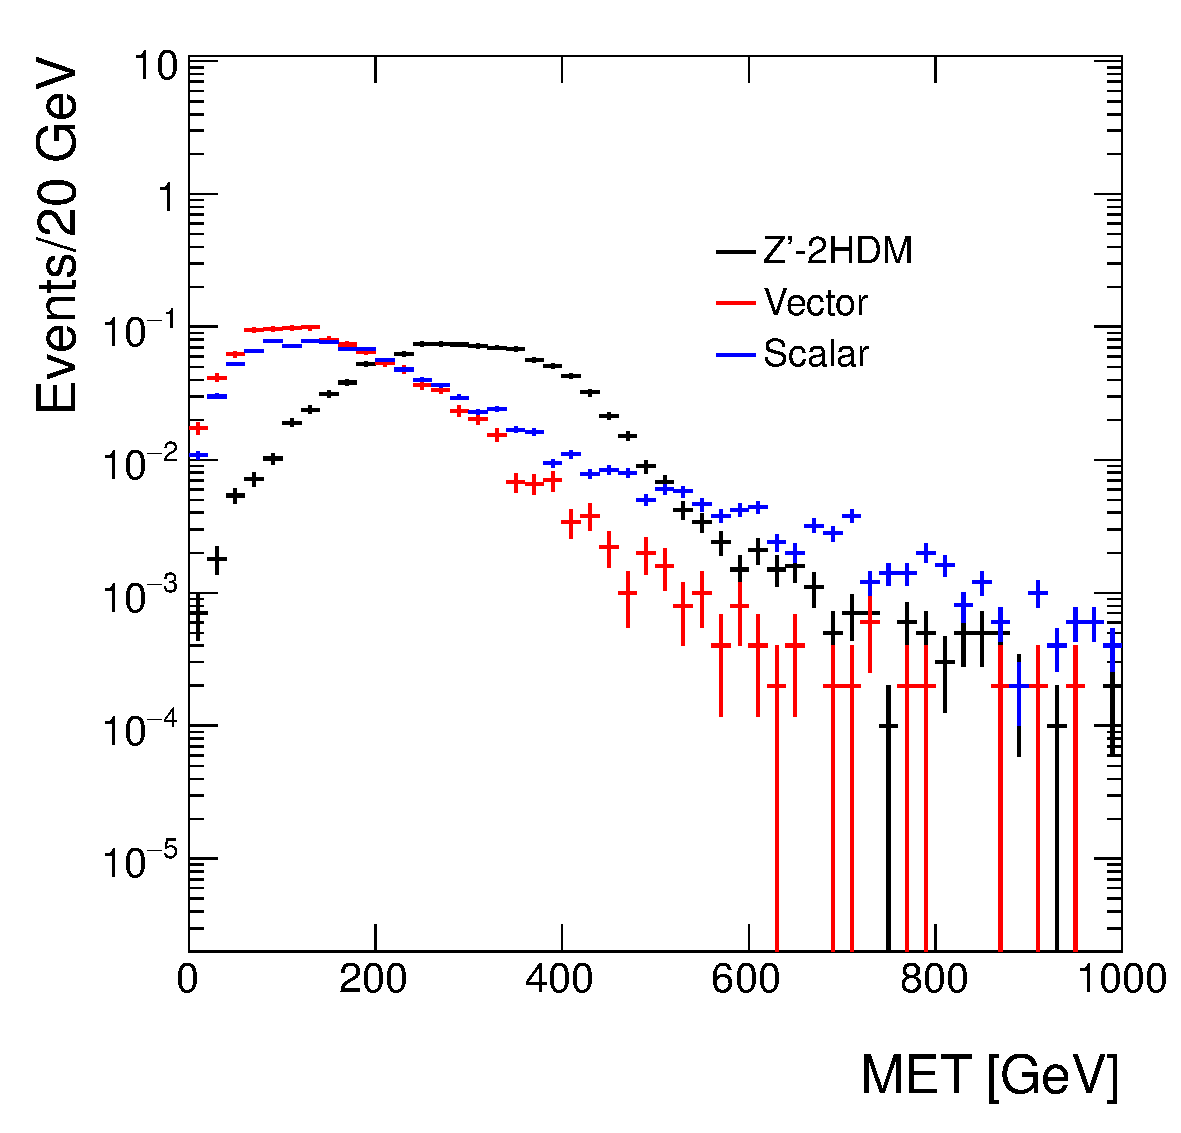
\includegraphics[width=0.47\linewidth]{figures/EW/monoH/models_cmp_MET_et_Log} \label{fig:met_cmp_high}
	}
	\subfloat[Low mediator mass]{
		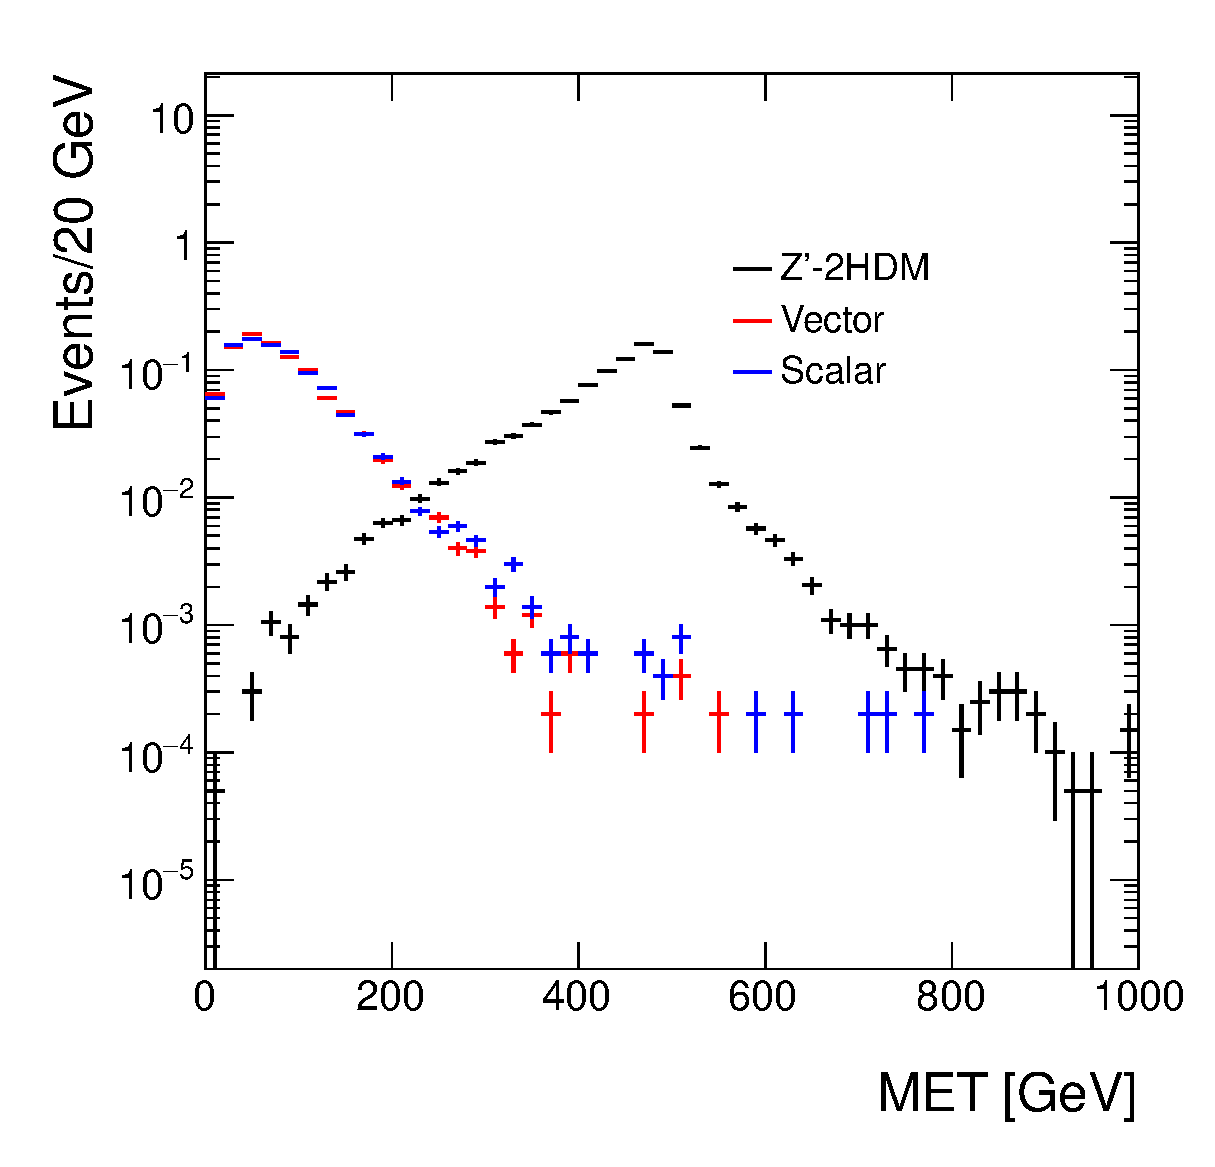
\includegraphics[width=0.47\linewidth]{figures/EW/monoH/models_cmp_low_MET_et_Log} \label{fig:met_cmp_low}
	}
	\caption{Comparison of the missing transverse momentum distributions at generator level in different 
		simplified models leading to a Higgs+MET signature. The model parameter settings are detailed in the text.
		\label{fig:METSimpMonoHiggs}}
\end{figure}


\paragraph{MET+Higgs from a baryonic Z'}

\textbf{[TODO for AB: add baryonic Higgs diagram]}

The first model, shown in Fig.~\ref{fig:monoH_baryonicZ} 
postulates a new gauge boson $Z'$ corresponding to a new $U(1)_B$ baryon 
number symmetry. The stable baryonic states included in this model are the DM candidate particles.
The mass of the $Z'$ boson is acquired through a baryonic Higgs $h_B$, which mixes with the 
SM Higgs boson. The interactions between the $Z'$, the quarks and the DM are described by 
the following Lagrangian:   

\be \label{ZprimeDM}
%%\mathscr{
	L =  g_q  \bar q \gamma^\mu q  Z_\mu' +
%
%\left\{ \begin{array}{cc}
%	%i  g_\chi  \chi^\dagger \smash{ \overset{\leftrightarrow}{\partial^\mu}}  \chi  Z^\prime_\mu + g_\chi^2 |\chi|^2 Z^\prime_\mu Z^{\prime\mu} & {\rm scalar}  
	 g_\chi  \bar\chi \gamma^\mu \chi Z_\mu' .
\ee

The quark couplings \gq are fixed to be equal to one third of the gauge coupling $g_B$, 
while the DM coupling to the $Z'$ are proportional to the baryon number and to the gauge coupling 
($g_{chi} = B g_B$). No leptonic couples of the $Z'$ are allowed, thus evading dilepton constraints. 
After incorporating the mixing of the baryonic and SM Higgs bosons, this model is 
is described by the following Lagrangian term at energies below $m_{Z^\prime}$: 
 \be \label{U1Beft}
 L_{\rm eff} = - \frac{g_q g_\chi }{m_{Z^\prime}^2} \bar{q} \gamma^\mu q \bar\chi \gamma_\mu \chi \Big( 1 + \frac{g_{h Z^\prime Z^\prime} }{m_{Z^\prime}^2} h \Big) \, ,
 \ee

The first term of this equation gives rise to a term that is equivalent to the 
radiation of a jet (or another EW gauge boson) in the initial state. 
The second term describes the interaction between the $Z'$ and the SM Higgs boson,
via the coupling $g_{h Z^\prime Z^\prime} = \frac{m_Z'^2 sin\theta}{v_B}$, where
$sin\theta$ is the mixing angle between the Higgs and the $Z'$ and $v_B$ is the
Baryonic Higgs vev. 

\textbf{[TODO: 
	1- Mention sensitivity difference wrt monojet? 
	2- Mention why we don't consider the dark Z model?]}

\textit{Parameter scan} 

Overall, this model is described by six parameters:
\begin{enumerate}
	\item the mediator mass \mmed, (also referred to as $m_{Z'}$)
	\item mass of dark matter, $m_{DM}$
	\item coupling of $Z'$ mediator to dark matter, \gdm
	\item coupling of the mediator to quarks, $g_q$
	\item mixing angle between baryonic Higgs and SM-like Higgs boson, $\sin\theta$
	\item coupling of the mediator to SM-like Higgs boson, $g_{hZ'Z'}$
\end{enumerate}
The width of the mediator is calculated using all possible decays, 
namely to quarks, to pairs of DM particles if kinematically allowed, 

The dependence of the missing transverse momentum (MET) on the model parameters 
is studied by varying the parameters one at a time. The variation of parameters 
other than $m_{med}$ and $m_{DM}$ does not result in significant 
variations of the MET spectrum, as shown in Figures~\ref{fig:metVectorCoupling}. 
Figure~\ref{fig:metVectorMass} shows that for an on-shell mediator, 
varying $m_{DM}$ with the other parameters fixed does not affect the MET distribution, while 
the distribution broadens significantly in the case of an off-shell mediator. 
For this reason, the same grid in \mmed, \mdm as for the vector mediator
of the jet+MET search (Table~\ref{tab:mDMmmedScan_VA}) is chosen as a starting point. 
The coupling between mediator and SM Higgs boson $g_{hZ'Z'}/ \mmed$ and the mediator-DM coupling \gdm are fixed to 1, the 
mediator-quark $g_{q}$ coupling is fixed to 1/3. Other parameter values can be recasted starting from the results
for those model parameters.
More detailed studies are required to estimate the reach of the analysis with respect to all points in the grid
and therefore decide on a smaller set of grid points to be generated; 
those are left to the individual analyses. \textbf{[TODO: can we get sensitivity to all the points for all signatures?]}

\begin{figure}[hbpt!]
	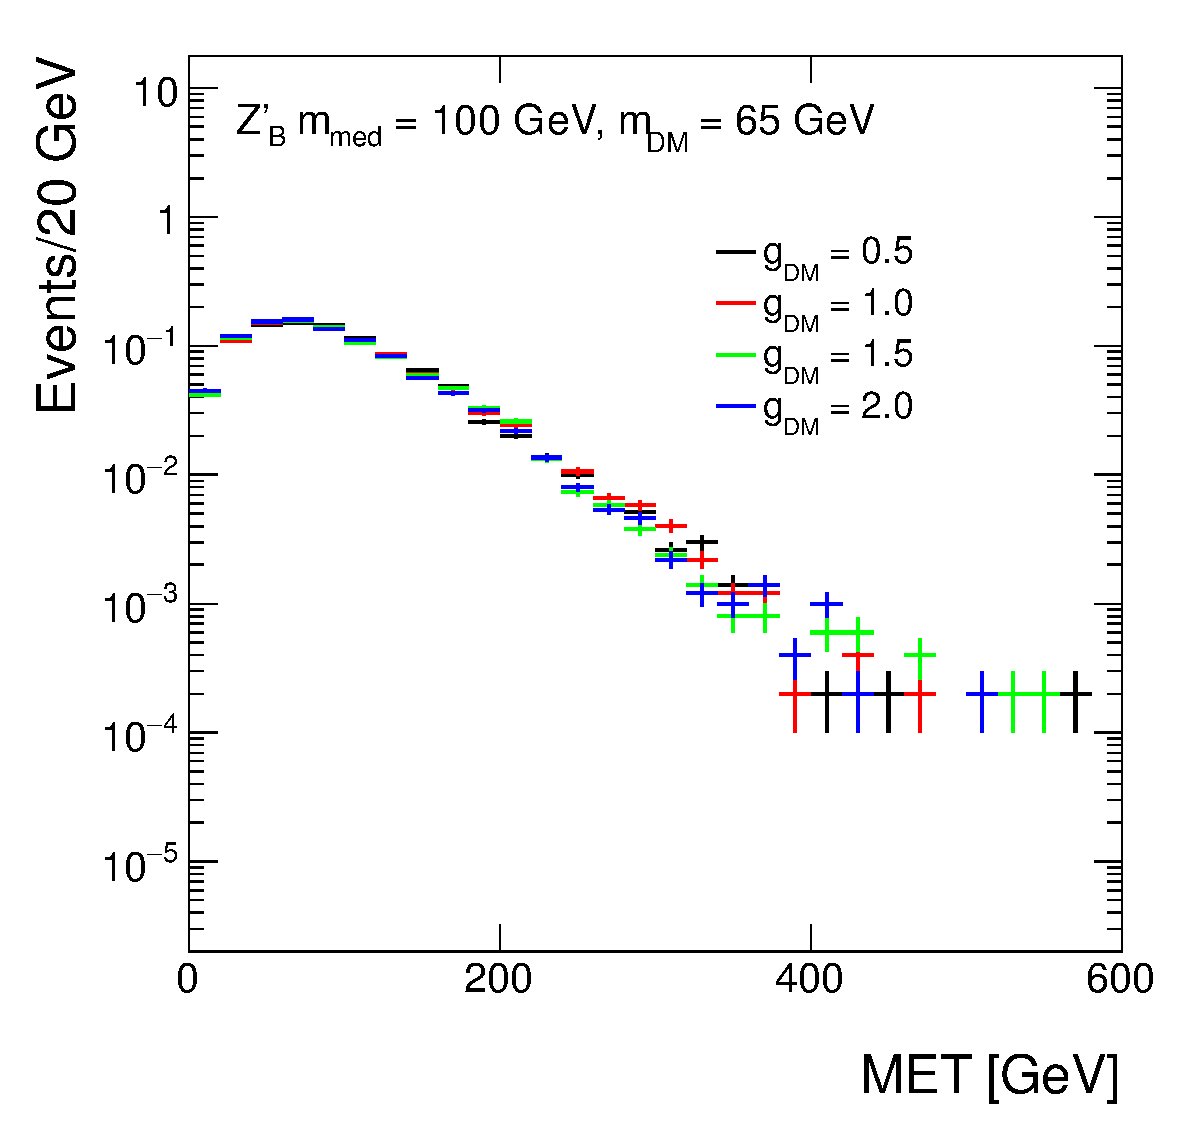
\includegraphics[width=0.49\linewidth]{figures/EW/monoH/z_gdm_MET_et_Log}
	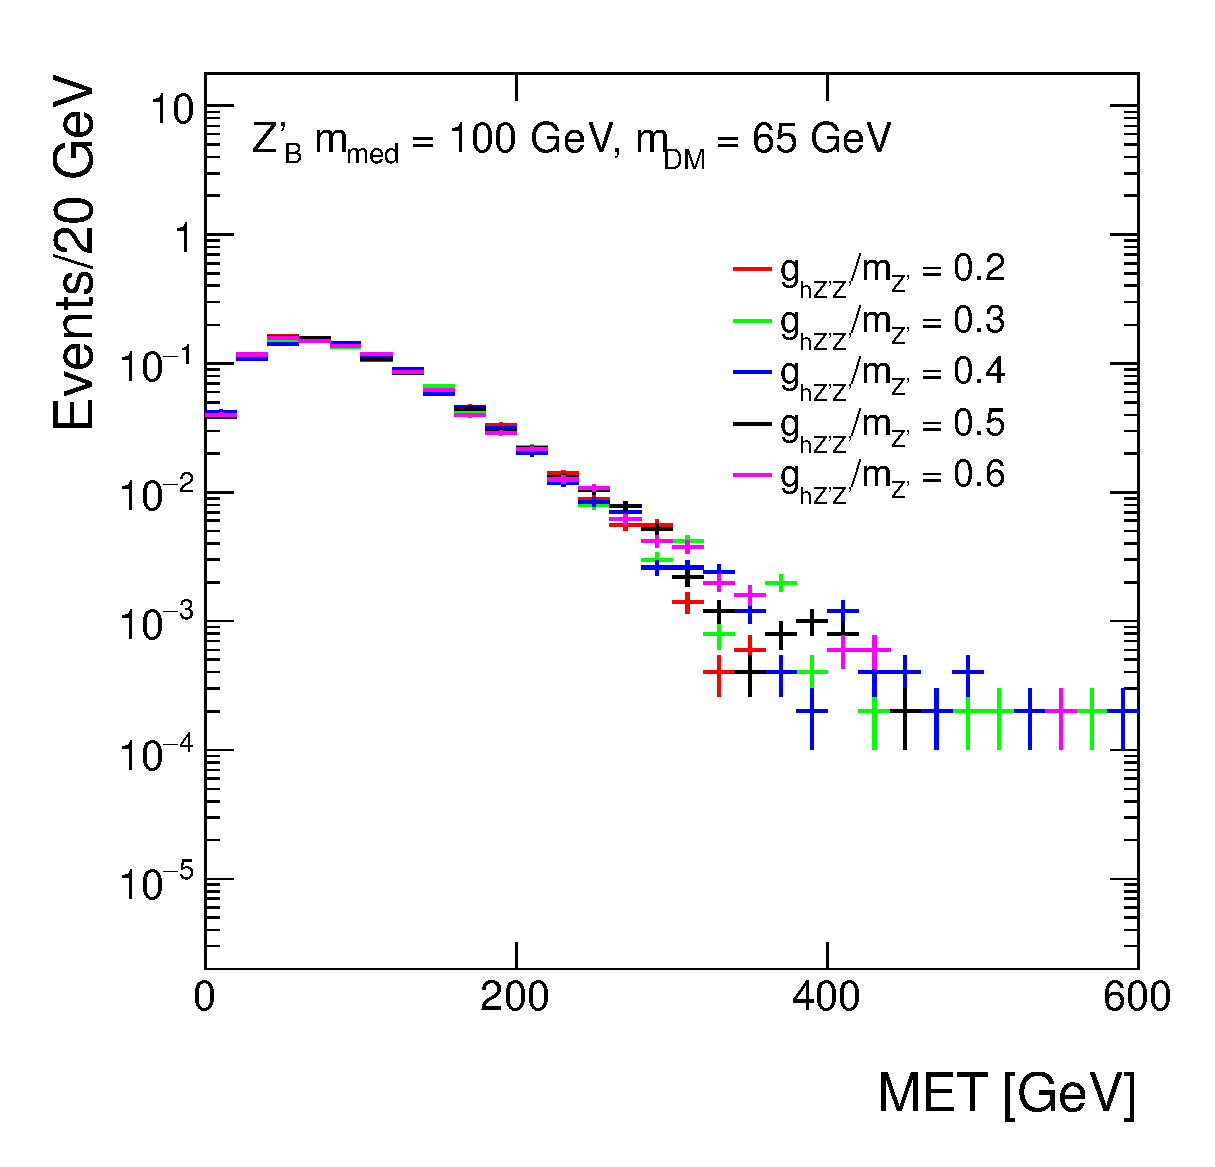
\includegraphics[width=0.49\linewidth]{figures/EW/monoH/z_ratio_MET_et_Log}
	\caption{Missing transverse momentum distributions at generator level in the vector 
		mediator scenario for different values of: the mediator-dark matter coupling \gdm (left),
		and the coupling between the mediator and the SM-like Higgs boson, scaled by the mediator mass, 
		$g_{hZ'Z'}/m_{Z'}$ (right).
		\label{fig:metVectorCoupling}}
\end{figure}

\begin{figure}[hbpt!]
	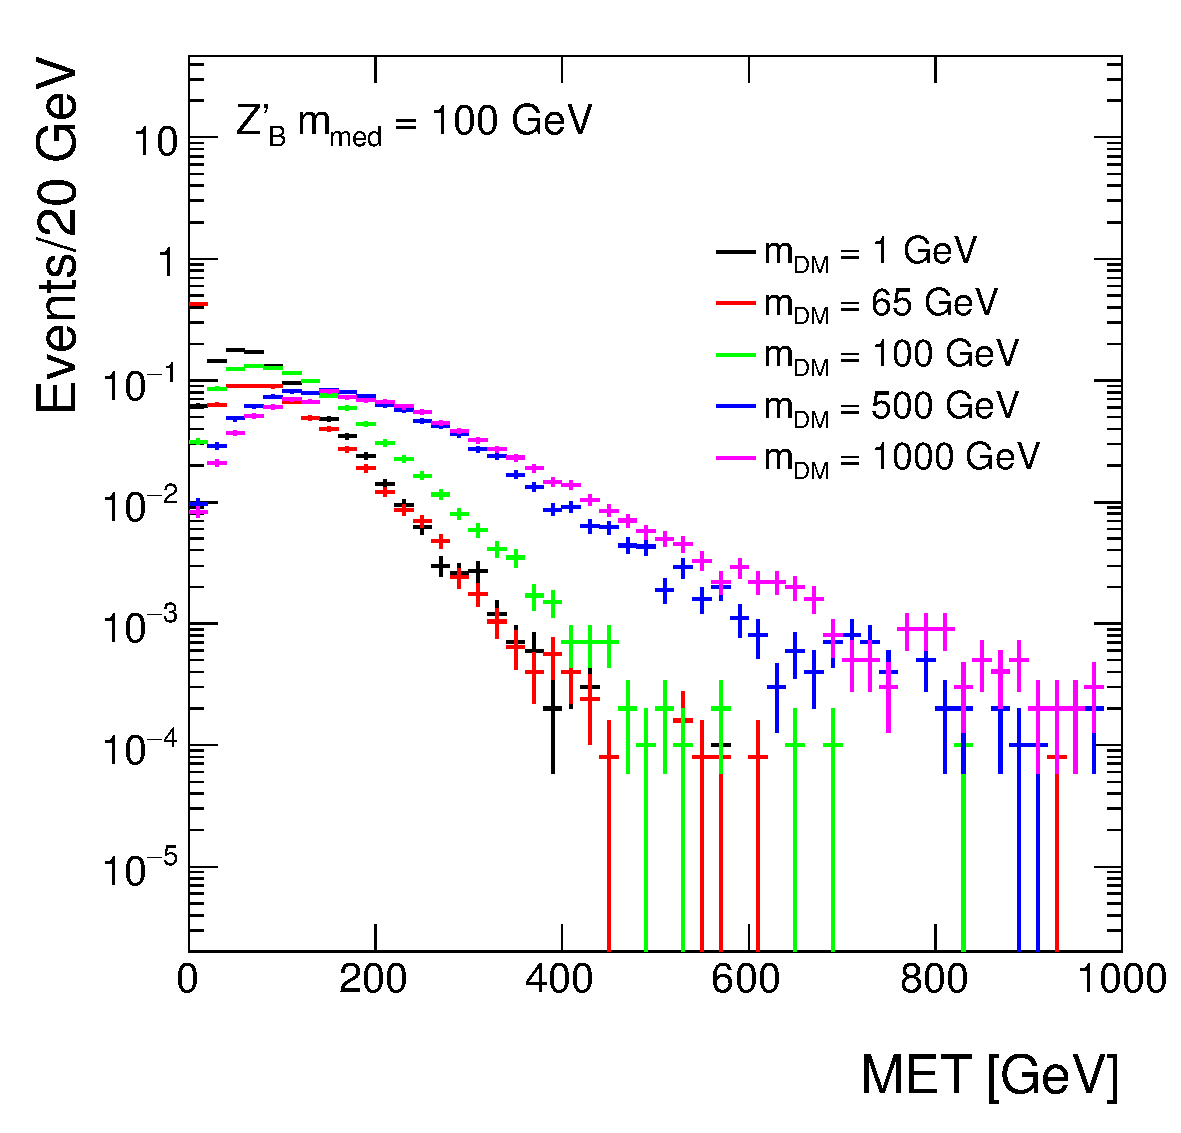
\includegraphics[width=0.49\linewidth]{figures/EW/monoH/zprime_100_MET_et_Log}
	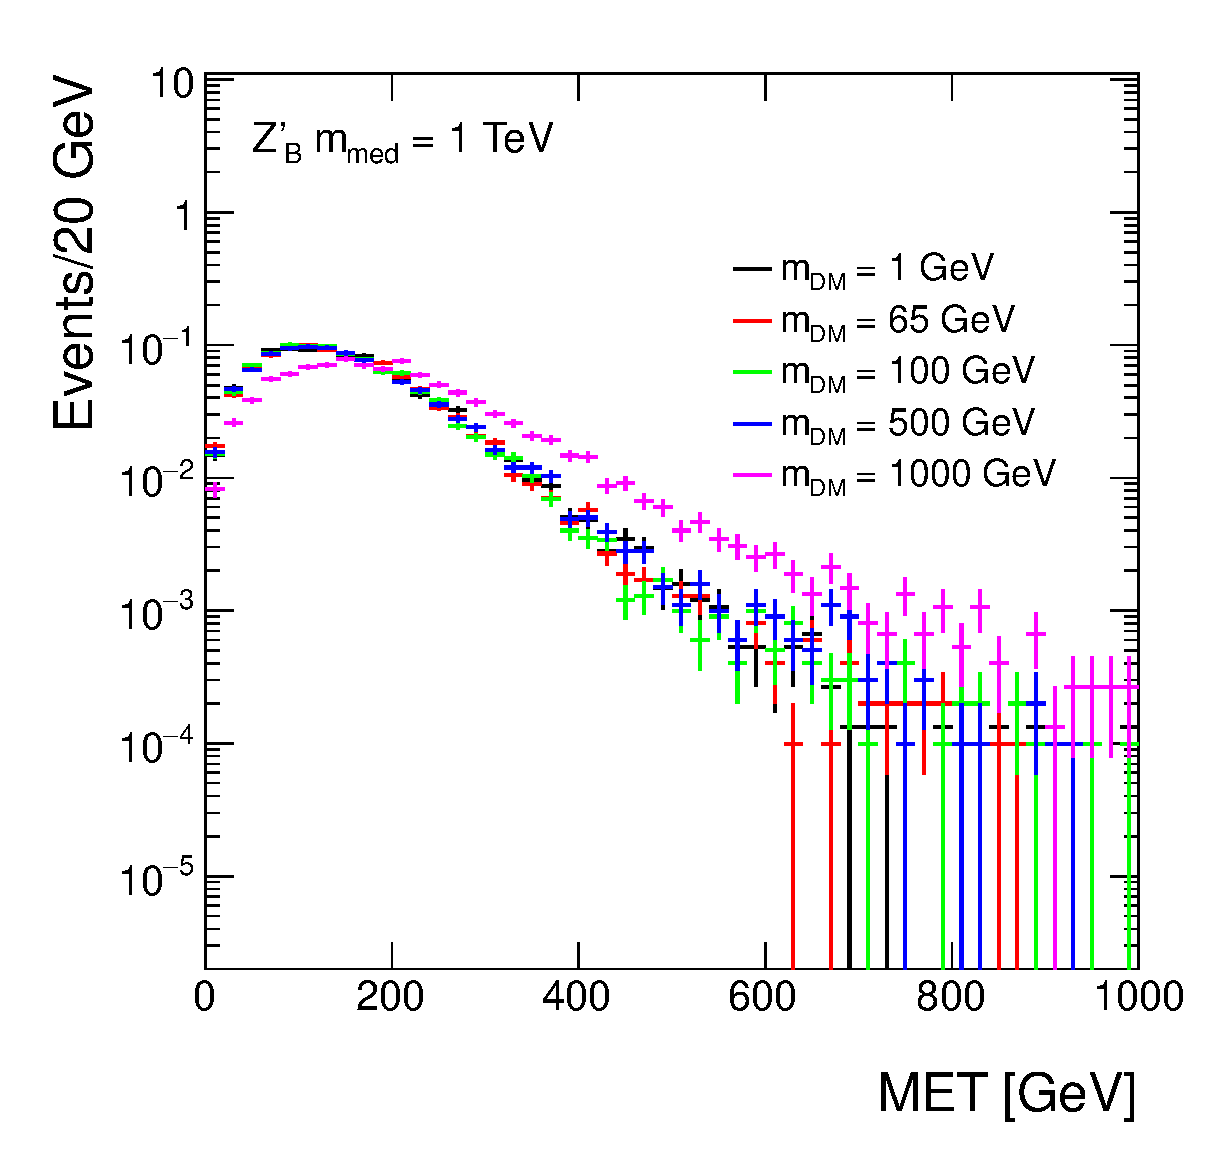
\includegraphics[width=0.49\linewidth]{figures/EW/monoH/zprime_1000_MET_et_Log}
	\caption{Missing transverse momentum distributions at generator level in the vector 
		mediator scenario: for different values of the dark matter mass $m_{DM}$ 
		and a mediator mass of \mmed = 100 GeV (left) and \mmed = 1 TeV (right).
		\label{fig:metVectorMass} }
\end{figure}

\textit{Cross-section scaling (to be added)}

\textit{Model implementation}

\textbf{[SVN repo and MG details to be added here]} 

\paragraph{MET+Higgs from a scalar mediator}

A real scalar singlet $S$ coupling to DM can be introduced as a portal between SM and the dark sector 
through the Higgs field. The new scalar mixes with the SM Higgs boson, and couples to DM through a Yukawa term $y_\chi$. 
The relevant Lagrangian terms for this model are: 

\be \label{LintScalar2}
L \supset - y_\chi \bar\chi \chi (  cos\theta S - sin\theta h ) - \frac{m_q}{v} \bar q q (cos\theta h + sin\theta S )  \,
\ee

where $\theta$ is the mixing angle between the Higgs boson and the new scalar. Mono-Higgs signals arise
\textbf{[TODO: add the Lagrangian explaining why $g_b$ is there]}

\textit{Parameter scan}

This model is described by five parameters: 

\begin{enumerate}
	\item the Yukawa coupling of heavy scalar to dark matter (DM), $g_{DM}$ (also referred to as $y_\chi$) 
	\item the mixing angle between heavy scalar and SM-like Higgs boson, $\sin\theta$
	\item the new physics coupling, $g_b$
	\item mass of heavy scalar, $m_{med}$ 
	\item mass of dark matter, $m_{DM}$ 
	%(also referred to as $m_{\chi}$)
\end{enumerate}

The mixing angle  is constrained from current Higgs data
to satisfy $\cos\theta = 1$ within 10\% and therefore $\sin\theta \lesssim 0.4$. This provides a starting point 
for the parameter scan in this model: we recommend to set $\sin\theta = 0.3$. 
Figure~\ref{fig:metScalarCoupling2} shows that
there is no dependence of the kinematics from the value of this angle, and different values can be obtained via rescaling
the results for this mixing angle according to the cross-section. It can also be observed from Figures~\ref{fig:metScalarMass} and~\ref{fig:metScalarCoupling} 
that the kinematics of this model follows that of the equivalent jet+MET model: only small changes are observed
in the on-shell region, while the relevant distributions diverge when the mediator is off-shell. 
For this reason, the same grid in \mmed, \mdm as for the scalar mediator
of the jet+MET search (Table~\ref{tab:mDMmmedScan_SP}) is chosen as a starting point. 
The Yukawa coupling to DM $y_{DM}$ is set to 1, the 
new physics coupling between scalar and SM Higgs $b$ = 3. Results for other values can be obtained via a 
rescaling of the results for these parameters. 
More detailed studies are required to estimate the reach of the analysis with respect to all points in the grid
and therefore decide on a smaller set of grid points to be generated; 
those are left to the individual analyses. \textbf{[TODO: can we get sensitivity to all the points for all signatures?]}

\begin{figure}[hbpt!]
	\begin{center}
		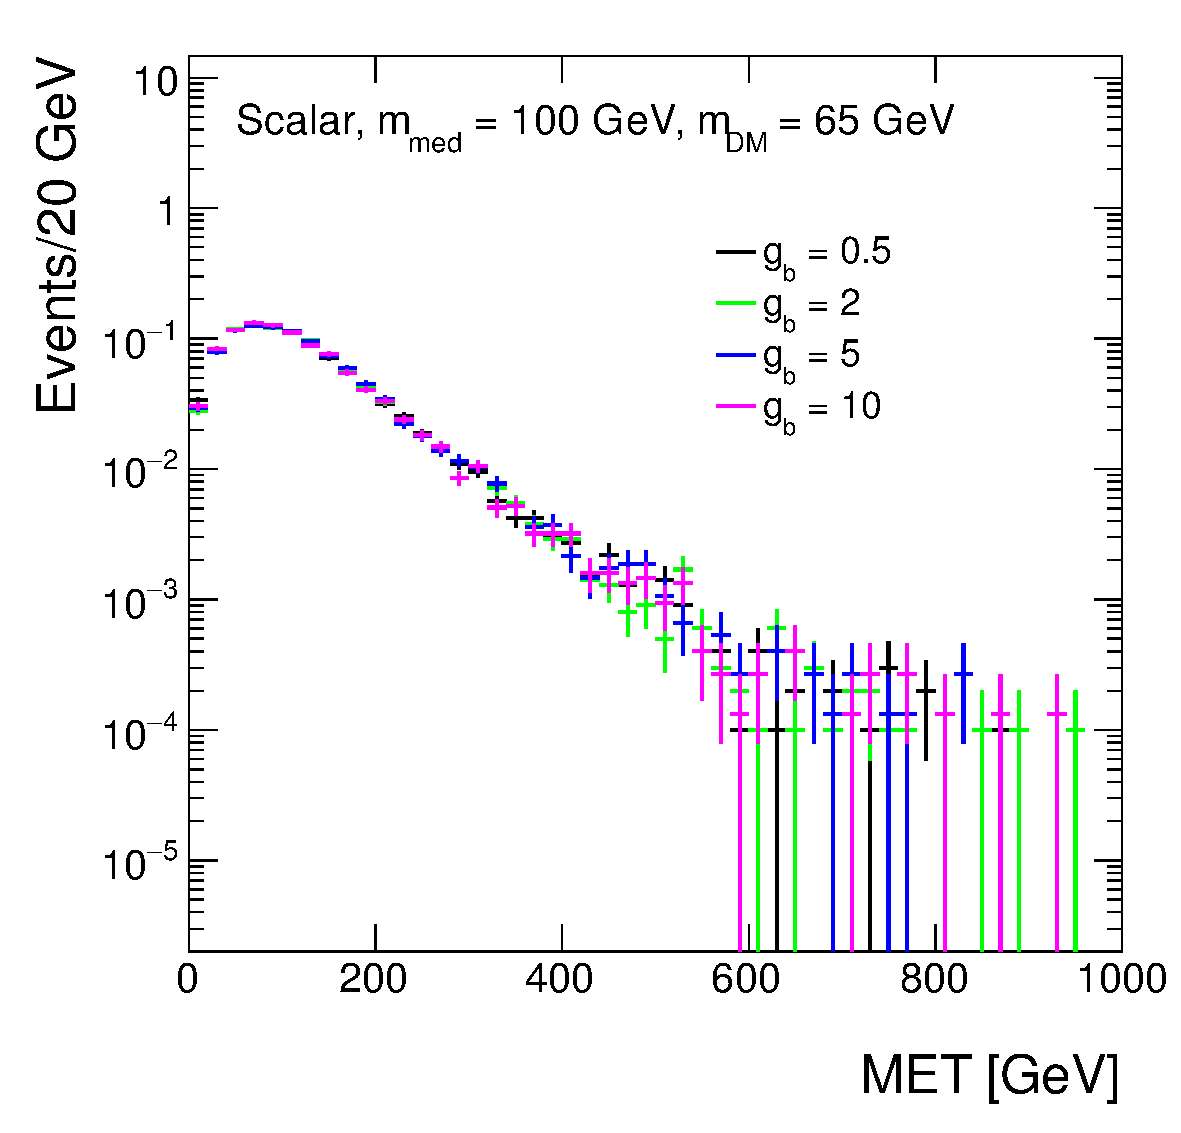
\includegraphics[width=0.49\linewidth]{figures/EW/monoH/s_gb_65_100_04_MET_et_Log}
		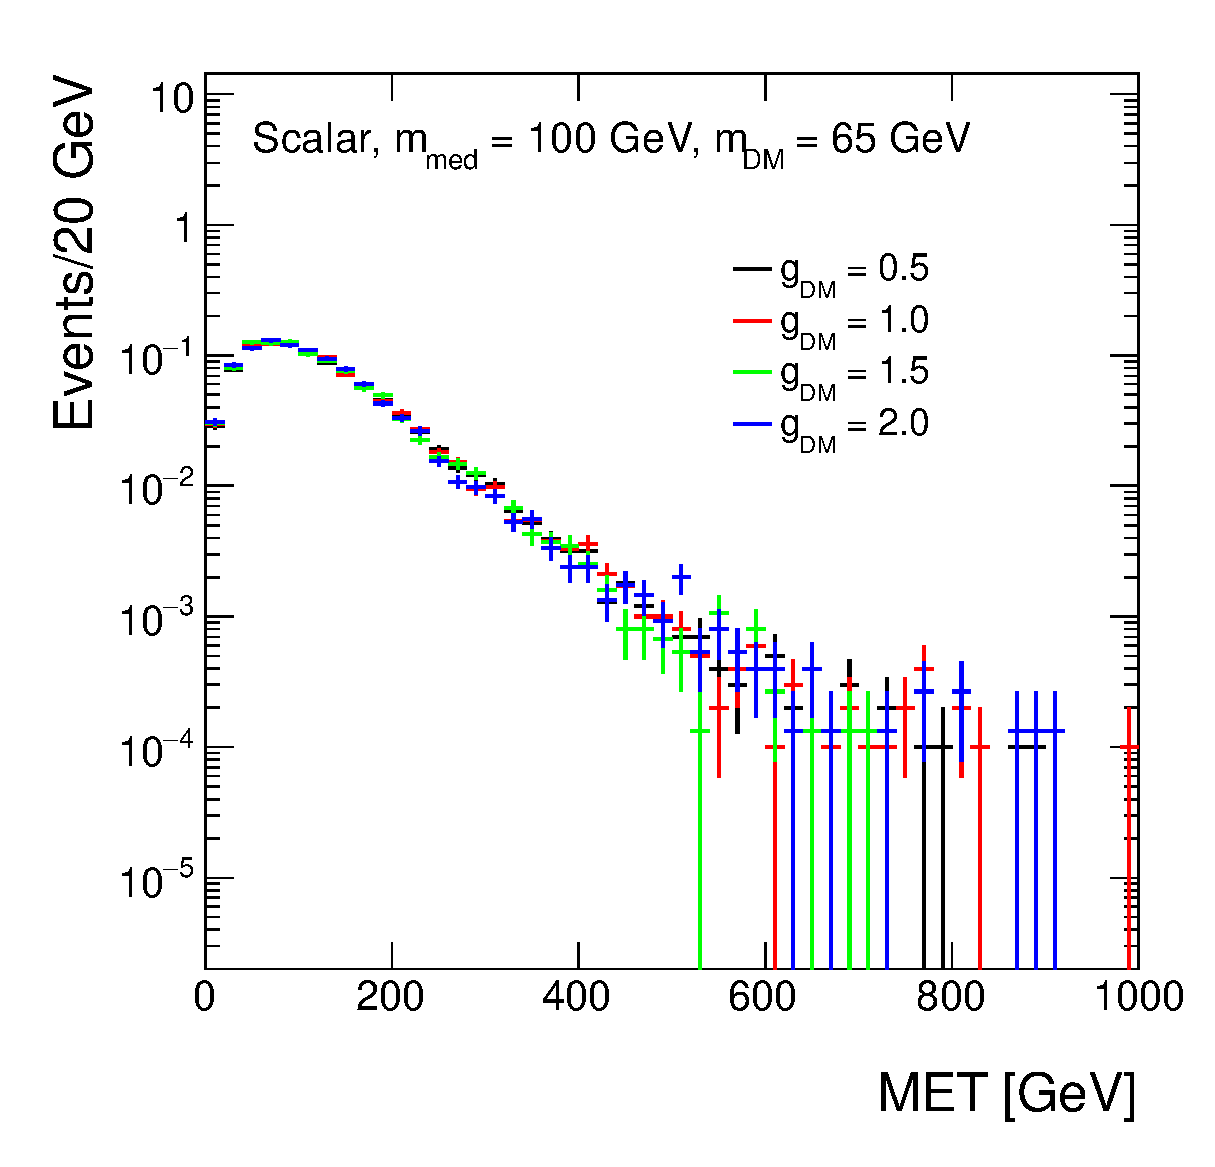
\includegraphics[width=0.49\linewidth]{figures/EW/monoH/s_gdm_MET_et_Log}
		\caption{Missing transverse momentum distributions at generator level in the scalar 
			mediator scenario, for different values of: the new physics coupling $g_b$ (left),
			and the mediator-dark matter coupling $g_{DM}$ (right).
			\label{fig:metScalarCoupling}}
	\end{center}
\end{figure}

\begin{figure}[hbpt!]
	\begin{center}
		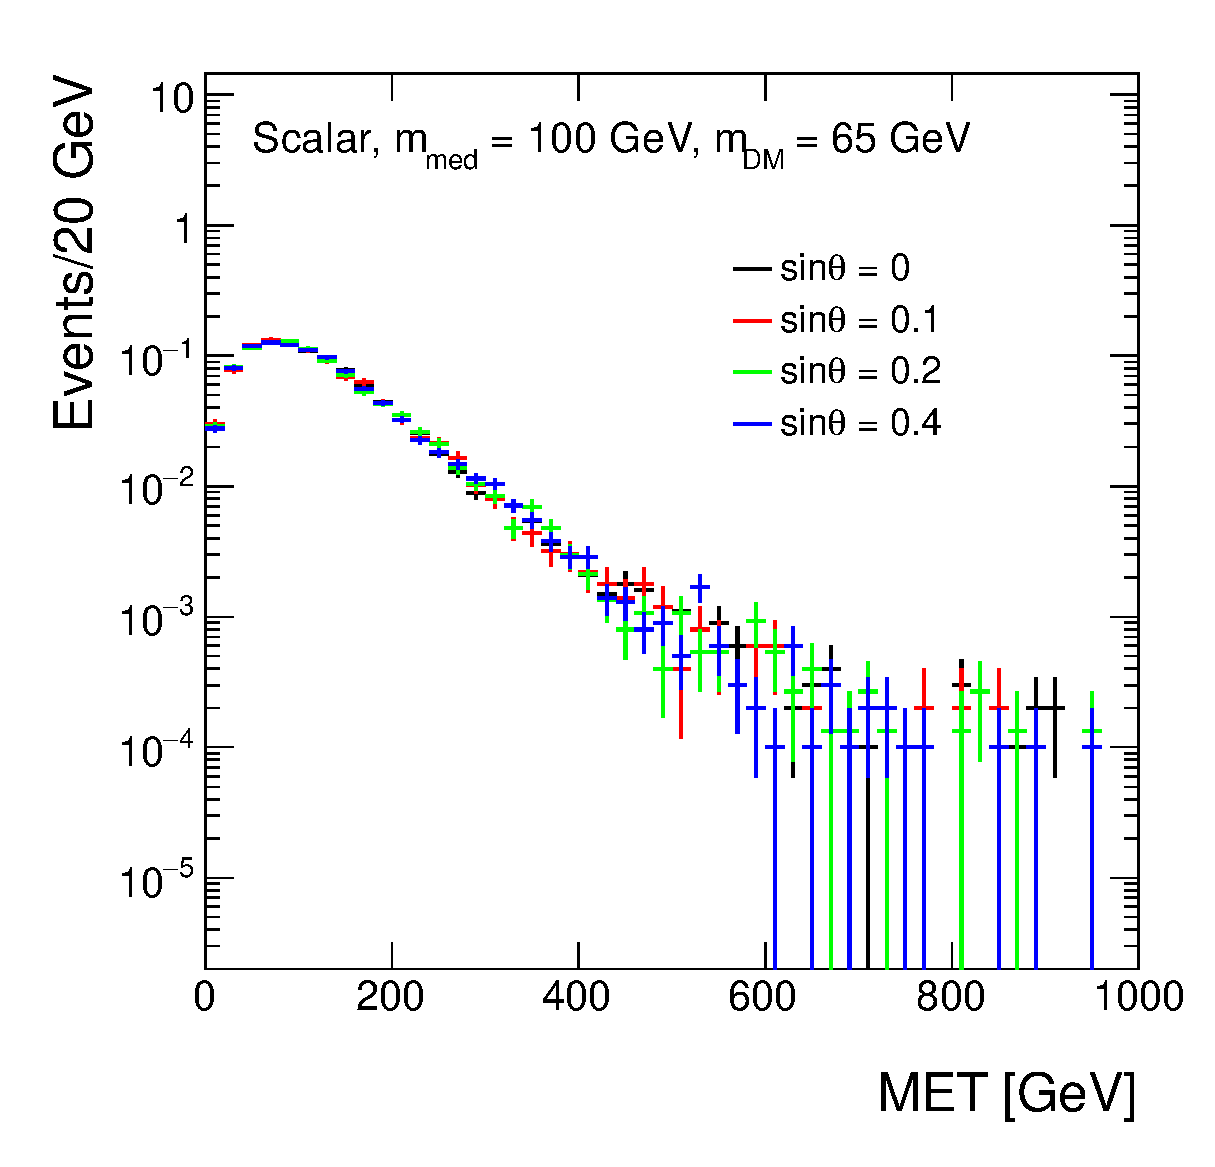
\includegraphics[width=0.49\linewidth]{figures/EW/monoH/s_theta_65_100_2_MET_et_Log}
		\caption{Missing transverse momentum distributions at generator level in the scalar 
			mediator scenario: for different values of the mixing angle $\sin\theta$.
			\label{fig:metScalarCoupling2} }
	\end{center}
\end{figure}

\begin{figure}[hbpt!]
	\begin{center}
		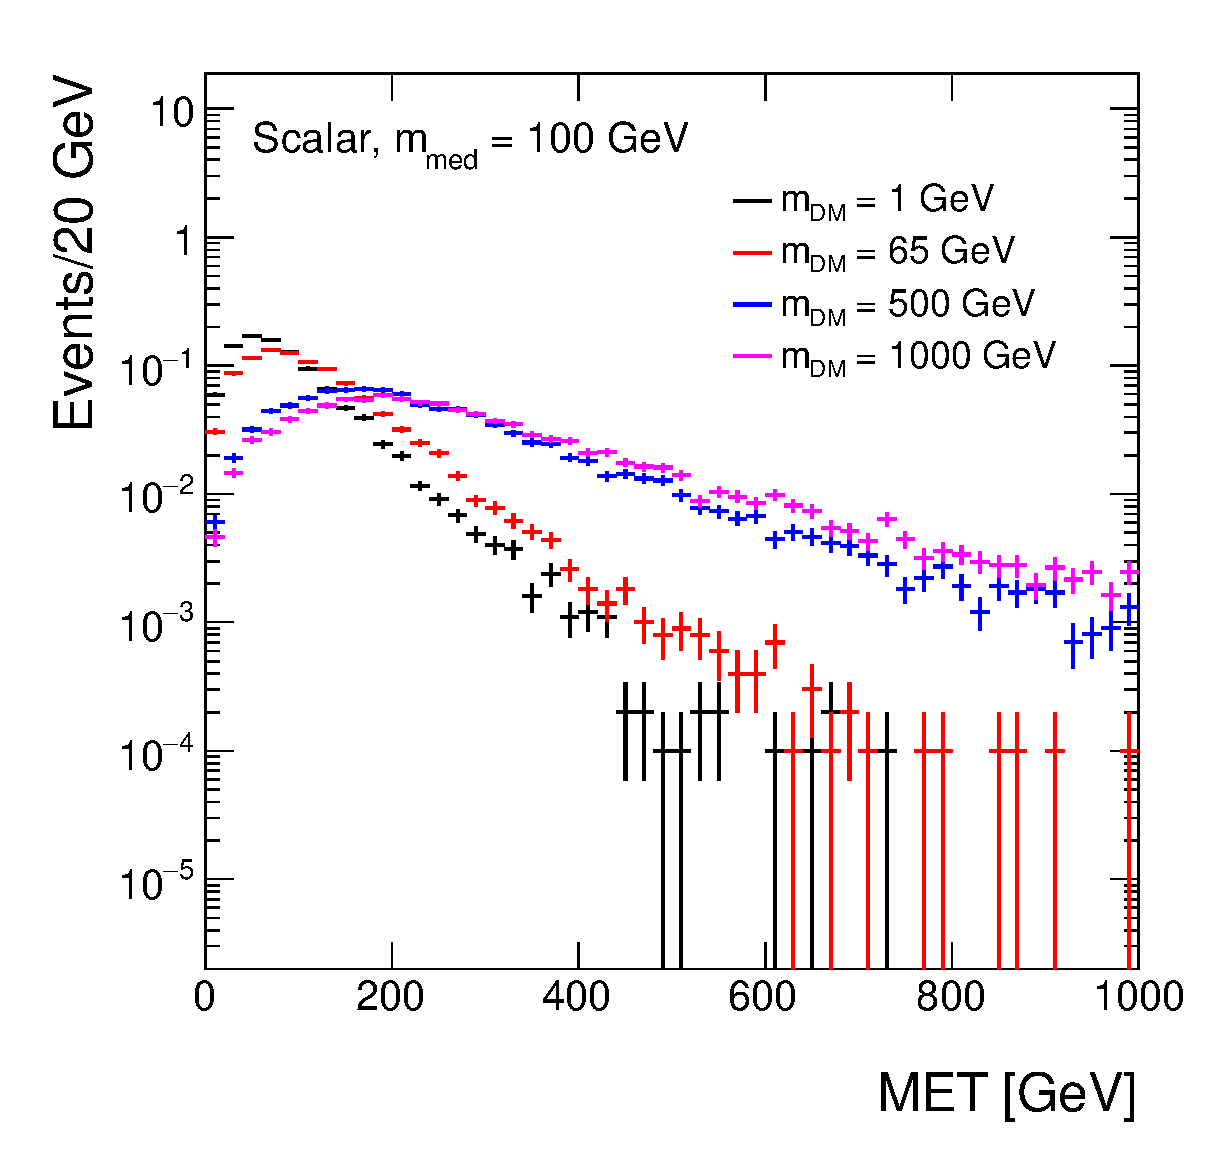
\includegraphics[width=0.49\linewidth]{figures/EW/monoH/scalar_100_MET_et_Log}
		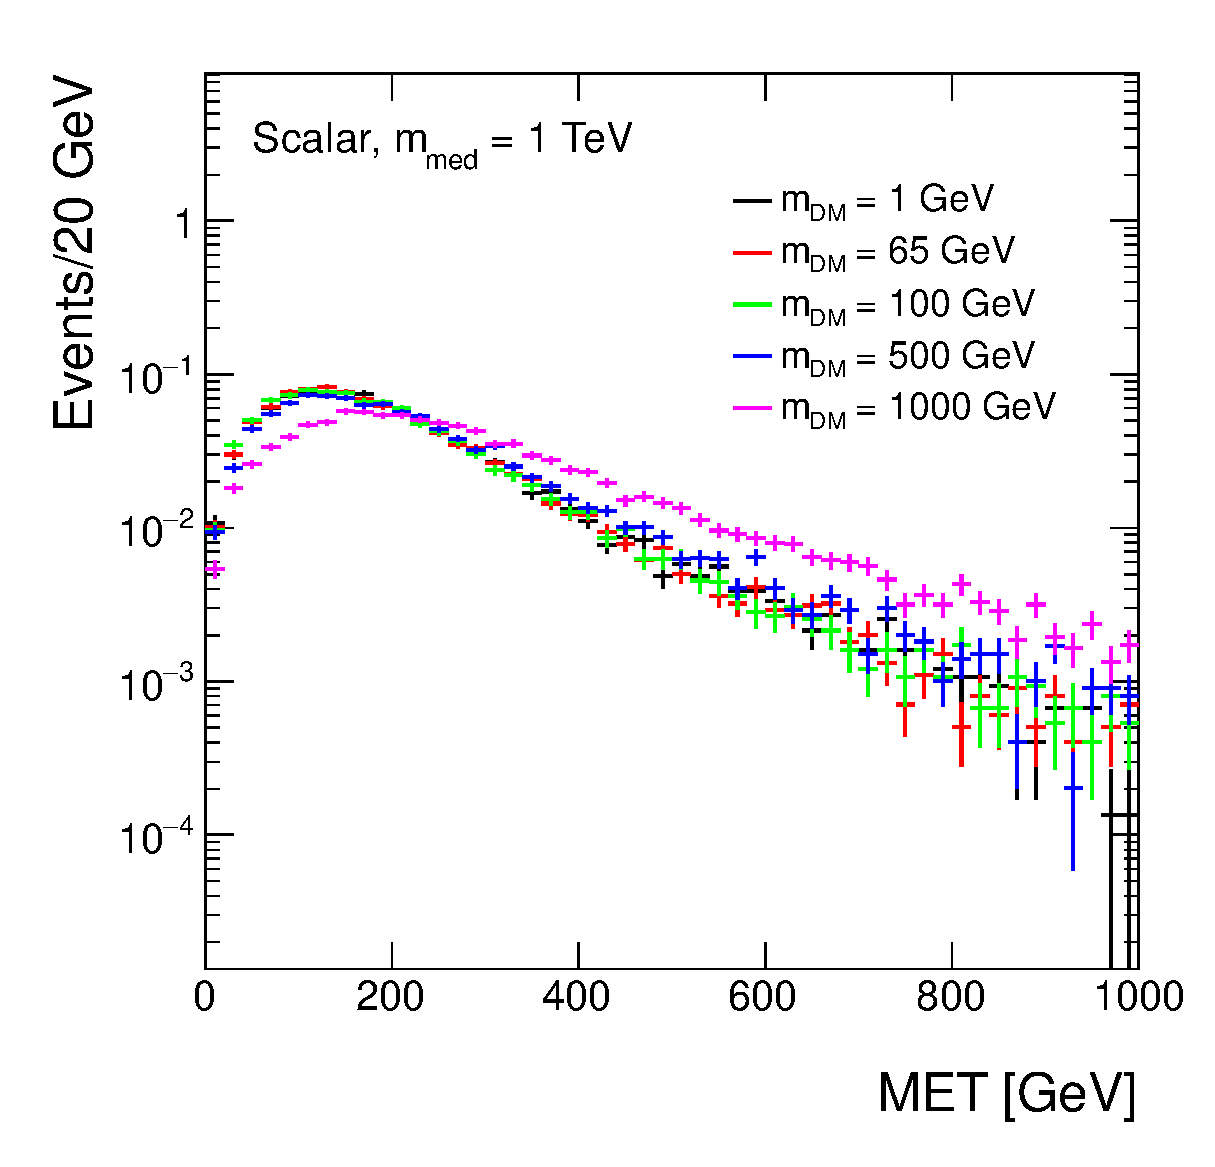
\includegraphics[width=0.49\linewidth]{figures/EW/monoH/scalar_1000_MET_et_Log}
		\caption{Missing transverse momentum distributions at generator level in the scalar 
			mediator scenario: for different values of the dark matter mass $m_{DM}$ 
			and a mediator mass of $m_{med}$ = 100 GeV (left) and $m_{med}$ = 1 TeV (right).
			\label{fig:metScalarMass}}
	\end{center}
\end{figure}

\textit{Cross-section scaling (to be added)}


\textit{Model implementation}

The Madgraph parameter cards can be found on the Forum repository. In this model, the contribution
from the $gghS$ box is included through an effective Lagrangian evaluated in the large $m_t$ limit. 
This may overestimate the rates of $h + \missET$ signal~\cite{Haisch:2012kf}, but a full evaluation
is left to future studies. The parton shower for these models is implemented in Pythia. 
It is recommended to let Pythia decay the Higgs boson, in order to make the BR consistent with HDECAY. 

%%%
\paragraph{Higgs+MET signal from 2HDM model with a Z' and a new pseudoscalar}

In this simplified model, a new $Z'$ resonance decays to a Higgs plus an intermediate state 
which in turn decays to a DM pair. Since a SM state decaying to DM would be highly constrained, 
we consider a two-Higgs doublet extension to the standard model (2HDM), 
where $Z'$ decays to $hA^0$, where $h$ is the SM Higgs boson with $m_h \sim 125$ GeV, 
and $A^0$ is a heavy pseudoscalar with a large branching ratio to dark matter. 
 
 This model comprises two doublets, where $\Phi_u$ couples to up-type quarks and $\Phi_d$ couples to down-type
 quarks and leptons:
 \begin{equation}
 -{\cal L} \supset  y_u Q \tilde \Phi_u \bar u + y_d Q \Phi_d \bar d + y_e L \Phi_d \bar e  + {\rm h.c.}
 \end{equation}
 
 After electroweak symmetry breaking, the Higgs doublets attain vevs $v_u$ and $v_d$, and in unitary gauge the doublets are parametrized as
 \begin{align}
 \Phi_d &= \frac{1}{\sqrt{2}}
 \begin{pmatrix}
 -\sin{\beta} \ H^+ \\ v_d - \sin{\alpha} \ h + \cos{\alpha} \ H - i \sin{\beta} \ A^0
 \end{pmatrix} 
 \quad , \nonumber \\
 \Phi_u &= \frac{1}{\sqrt{2}}
 \begin{pmatrix}
 \cos{\beta} \ H^+ \\ v_u + \cos{\alpha} \ h + \sin{\alpha} \ H + i \cos{\beta} \ A^0
 \end{pmatrix}
 \end{align}
 where $h,H$ are neutral CP-even scalars and $A^0$ is a neutral CP-odd scalar. 
 Furthermore, $\tan{\beta} \equiv v_u/v_d$, and $\alpha$ is the mixing angle that diagonalizes the $h - H$ mass squared matrix.
  The remaining scalars $H, A^0, H^\pm$ are assumed to have masses around or above $300$ GeV, 
  respecting $b \to s \gamma$ constraints \cite{Branco:2011iw}. 
  We further take $\alpha = \beta - \pi/2$, the alignment limit where $h$ has SM-like couplings to fermions and 
  gauge bosons as per Ref\cite{Craig:2013hca}, and $\tan{\beta} \ge 0.3$ as implied from the perturbativity of the top Yukawa coupling. 
  %For the $ b \bar{b}$ decay channel, the signature of the signal we are searching for is a pair of boosted WIMPs recoiling against two $b$ jets. 
 
 The Higgs vevs lead to $Z-Z'$ mass mixing. Diagonalizing the gauge
 boson mass matrix, the tree-level masses of the $Z$ and $Z'$ bosons are given by
 \begin{align}
 M_Z^2 &\approx ( M_{Z}^0)^2  - \epsilon^2 \left[( M_{Z'}^0)^2 - ( M_{Z}^0)^2 \right] \nonumber \\
 M_{Z'}^2 &\approx ( M_{Z'}^0)^2 + \epsilon^2 \left[( M_{Z'}^0)^2 - ( M_{Z}^0)^2 \right]
 \quad ,
 \label{eq:Zpmasses}
 \end{align}
 where $(M_Z^0)^2 = g^2(v_d^2+ v_u^2)/(4\cos^2{\theta_w}) $ and
 $(M_{Z'}^0)^2 = g_z^2 ( z_d^2 v_d^2 + z_u^2 v_u^2 + z_\phi^2
 v_\phi^2)$ are the mass-squared values in the absence of mixing. The
 result above is accurate to order $\epsilon^2$, where $\epsilon$ is
 a small mixing parameter given by
 \begin{align}
 \epsilon & \equiv \frac{1}{M_{Z'}^2 - M_Z^2} \frac{g g_z}{2 \cos{\theta_w}} ( z_d v_d^2 + z_u v_u^2) \nonumber \\
 & =  \frac{(M_Z^0)^2}{M_{Z'}^2 - M_Z^2} \frac{2 g_z \cos \theta_w}{g}  z_u \sin^2 \beta.
 \label{eq:epsilon}
 \quad
 \end{align}
 
 \textit{Parameter scan}
 
 The model is described by five parameters:
 \begin{itemize}
 	\item the pseudoscalar mass $M_{A^0}$,
 	\item the DM mass \mdm, 	 
 	\item the $Z'$ mass, $M_{Z'}$,
    \item $\tan{\beta} (\equiv v_u/v_d)$,
 	\item the $Z'$ coupling strength $g_z$. 
 \end{itemize}

 To study the signal production and kinematic dependencies on these parameters, 
 we produced signal samples varying each of the five parameters through 
 MadGraph for the matrix element, PYTHIA for the parton shower, and DELPHES\cite{deFavereau:2013fsa} 
for a parameterized detector-level simulation.
 
 As seen in Fig.~\ref{fig:DMH_tanbeta}, variations of $\tan{\beta}$ does not lead to any kinematic 
 difference and the production cross section simply scales as a function of $\tan{\beta}$. Hence 
we recommend to fix $\tan{\beta}$ to unity in signal generation. 

%\begin{figure}[hbpt!]
%	\centering
%	\subfloat[High mediator mass]{
%		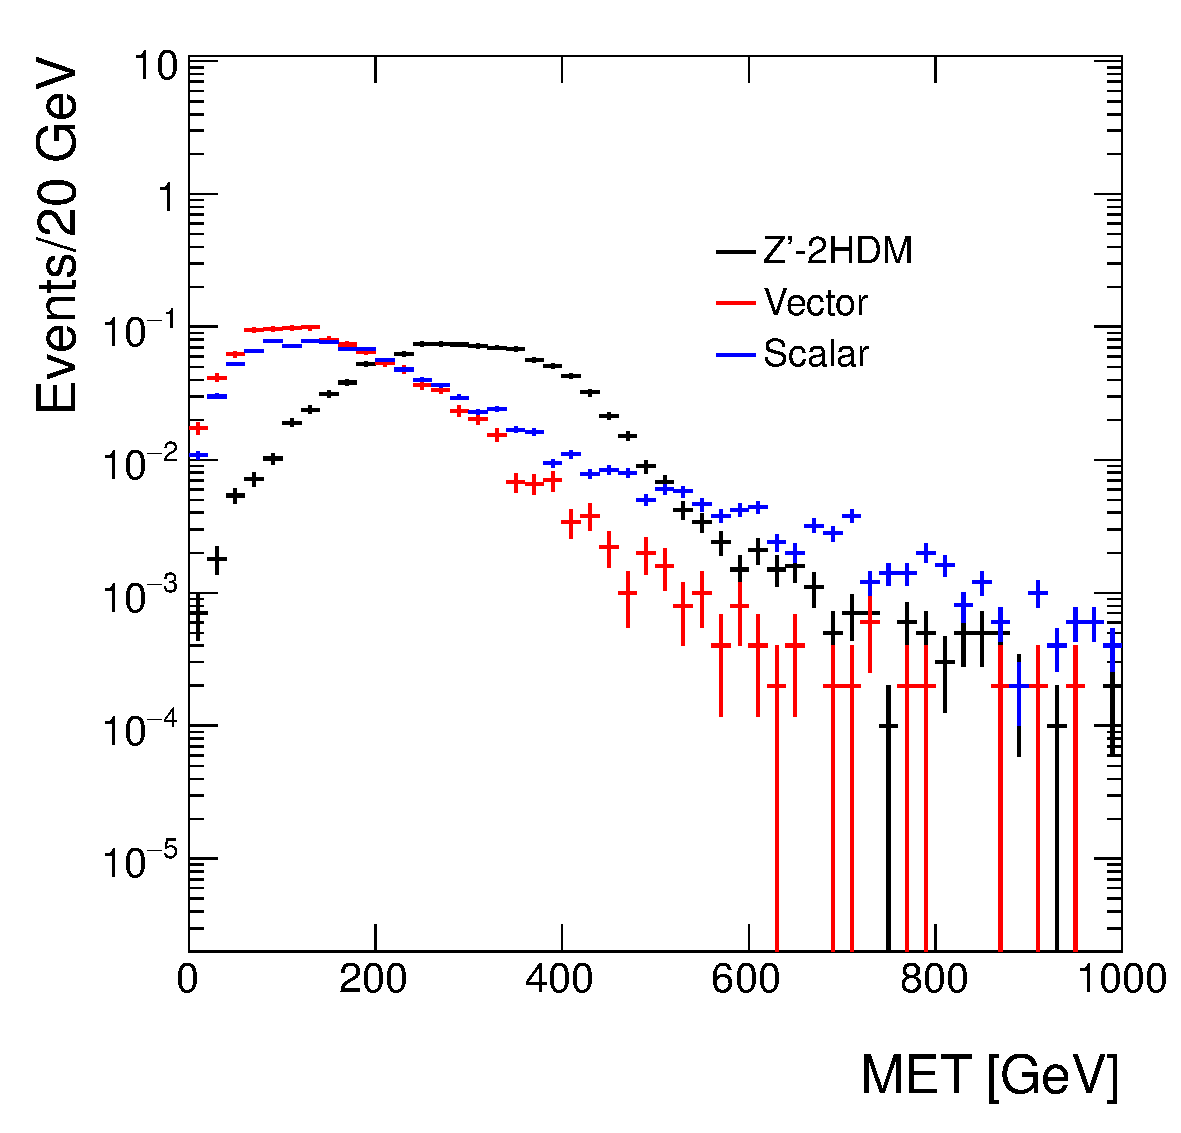
\includegraphics[width=0.47\linewidth]{figures/EW/monoH/models_cmp_MET_et_Log} \label{fig:met_cmp_high}
%	}
%	\subfloat[Low mediator mass]{
%		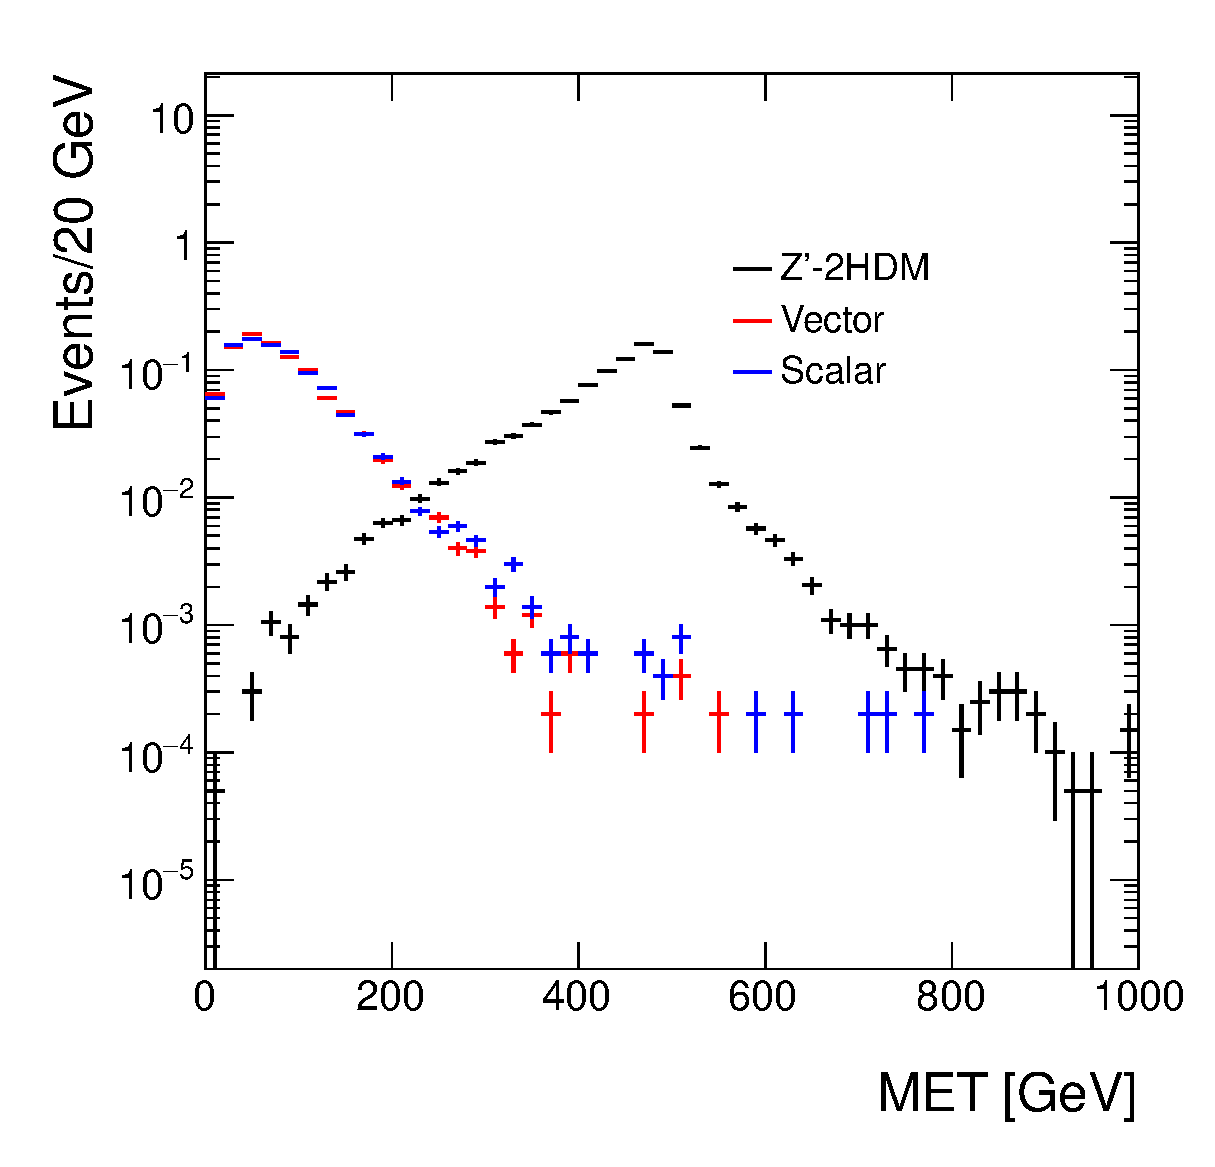
\includegraphics[width=0.47\linewidth]{figures/EW/monoH/models_cmp_low_MET_et_Log} \label{fig:met_cmp_low}
%	}
%	\caption{Comparison of the missing transverse momentum distributions at generator level in different 
%		simplified models leading to a Higgs+MET signature. The model parameter settings are detailed in the text.
%		\label{fig:METSimpMonoHiggs}}
%\end{figure}

\begin{figure}[h!]
\centering
\begin{minipage}{0.49\textwidth}
	\centering 
	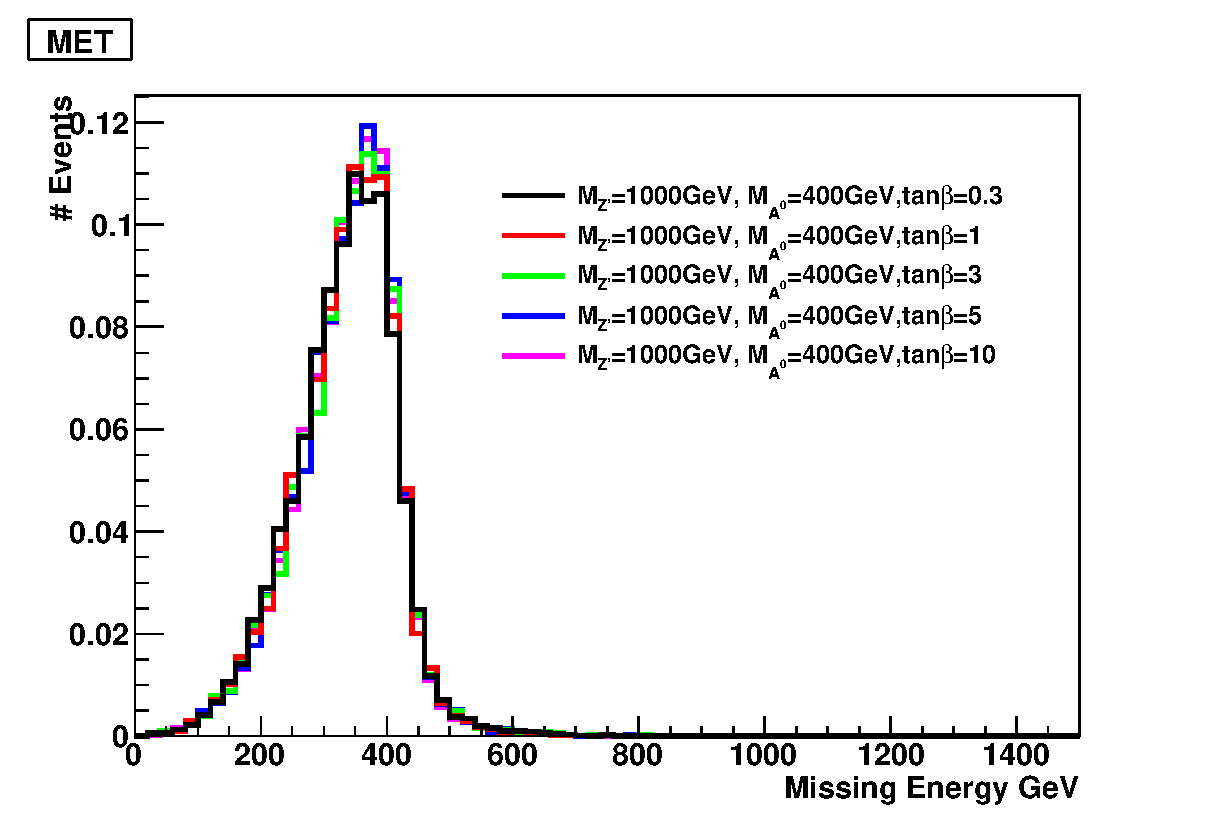
\includegraphics[scale=0.45]{figures/EW/monoH/2hdm/hxx_zp1000dm10gz01_met}
\end{minipage}
\hfill
\begin{minipage}{0.49\textwidth}
	\centering 
	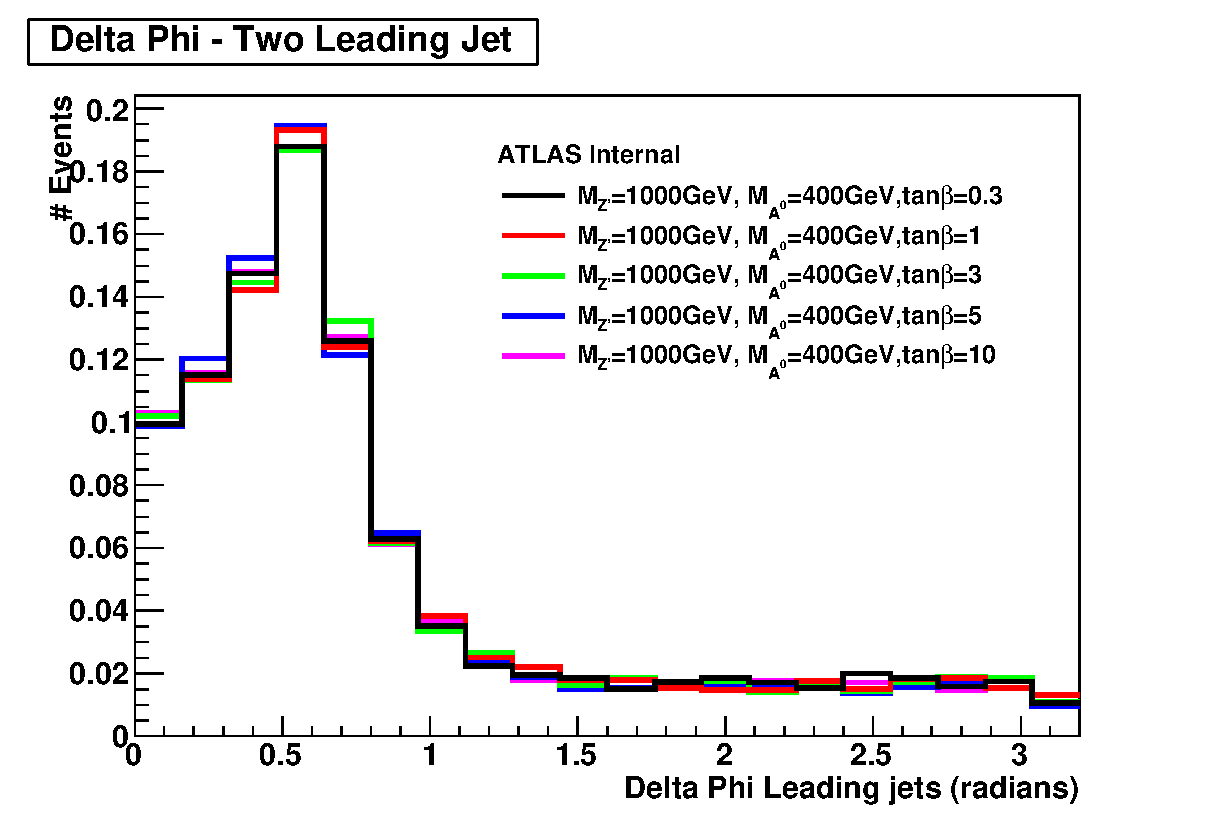
\includegraphics[scale=0.45]{figures/EW/monoH/2hdm/hxx_zp1000dm10gz01_dphi12}
\end{minipage}
\caption{Kinematic distributions of the signal process varying $\tan{\beta}$: no kinematic dependency on $\tan{\beta}$ is observed}
\label{fig:DMH_tanbeta}
\end{figure}

Similarly, variations of $g_z$ do not lead to any kinematic changes,
 and the production cross section scales as $(g_z)^2$, as the decay width for this process
to leading order in $\epsilon$ (Eq.~\ref{eq:epsilon}) is
\begin{equation}
\Gamma_{Z' \to hA^0} =  (g_z \cos \alpha \cos \beta)^2 \frac{|p|}{24 \pi} \frac{|p|^2}{M_{Z'}^2}.
\end{equation}
where the center of mass momentum for the decay products $|p| =
\frac{1}{2 M_{Z'}} \lambda^{1/2}(M_{Z'}^2,m_h^2, m_{A^0}^2)$, and
$\lambda$ is the K\"{a}llen triangle function.  
 
 %%CD UP TO HERE
 
 \textit{Model implementation}
 
 \textbf{[Ask Yangyang for model / check she hasn't sent it already.]}
%%%

%%This is left here in case we want to recommend EFT benchmarks?
% \begin{description}
%  \item[Vector interaction with vector-vector couplings (D5)]. For both jet+MET and boson+MET searches, the kinematic of this operator corresponds to that of couplings that are vector-axial (D7), axial-axial (D8) and axial-vector (D6). In the case of W boson radiation, the three coupling scenarios $\xi=1,0,-1$ should be investigated. This operator populates the high MET
%  \item[Tensor interaction (D9)]. As shown in Figure \textbf{[CD: add picture from Andy]}, this operator populates a higher MET range with respect to the other operators chosen.
%  \item[Scalar interaction (D1)]. This operator has the lowest cross-section and sensitivity at colliders in this final state, as DM production from light quarks via a scalar interaction is suppressed with respect to heavy quarks. However, it has the hardest MET spectrum of the EFT operators chosen, and results obtained using this operator as benchmark may be used for recasting signals with a similarly hard MET distribution.~\footnote{Q for Andy/M-E: ZZchichi max gamma: is it the same kinematics regardless of DM? See fig. 2 of ATLAS monoZ.}
% \end{description}
